\begin{figure}[t]
  \centering
  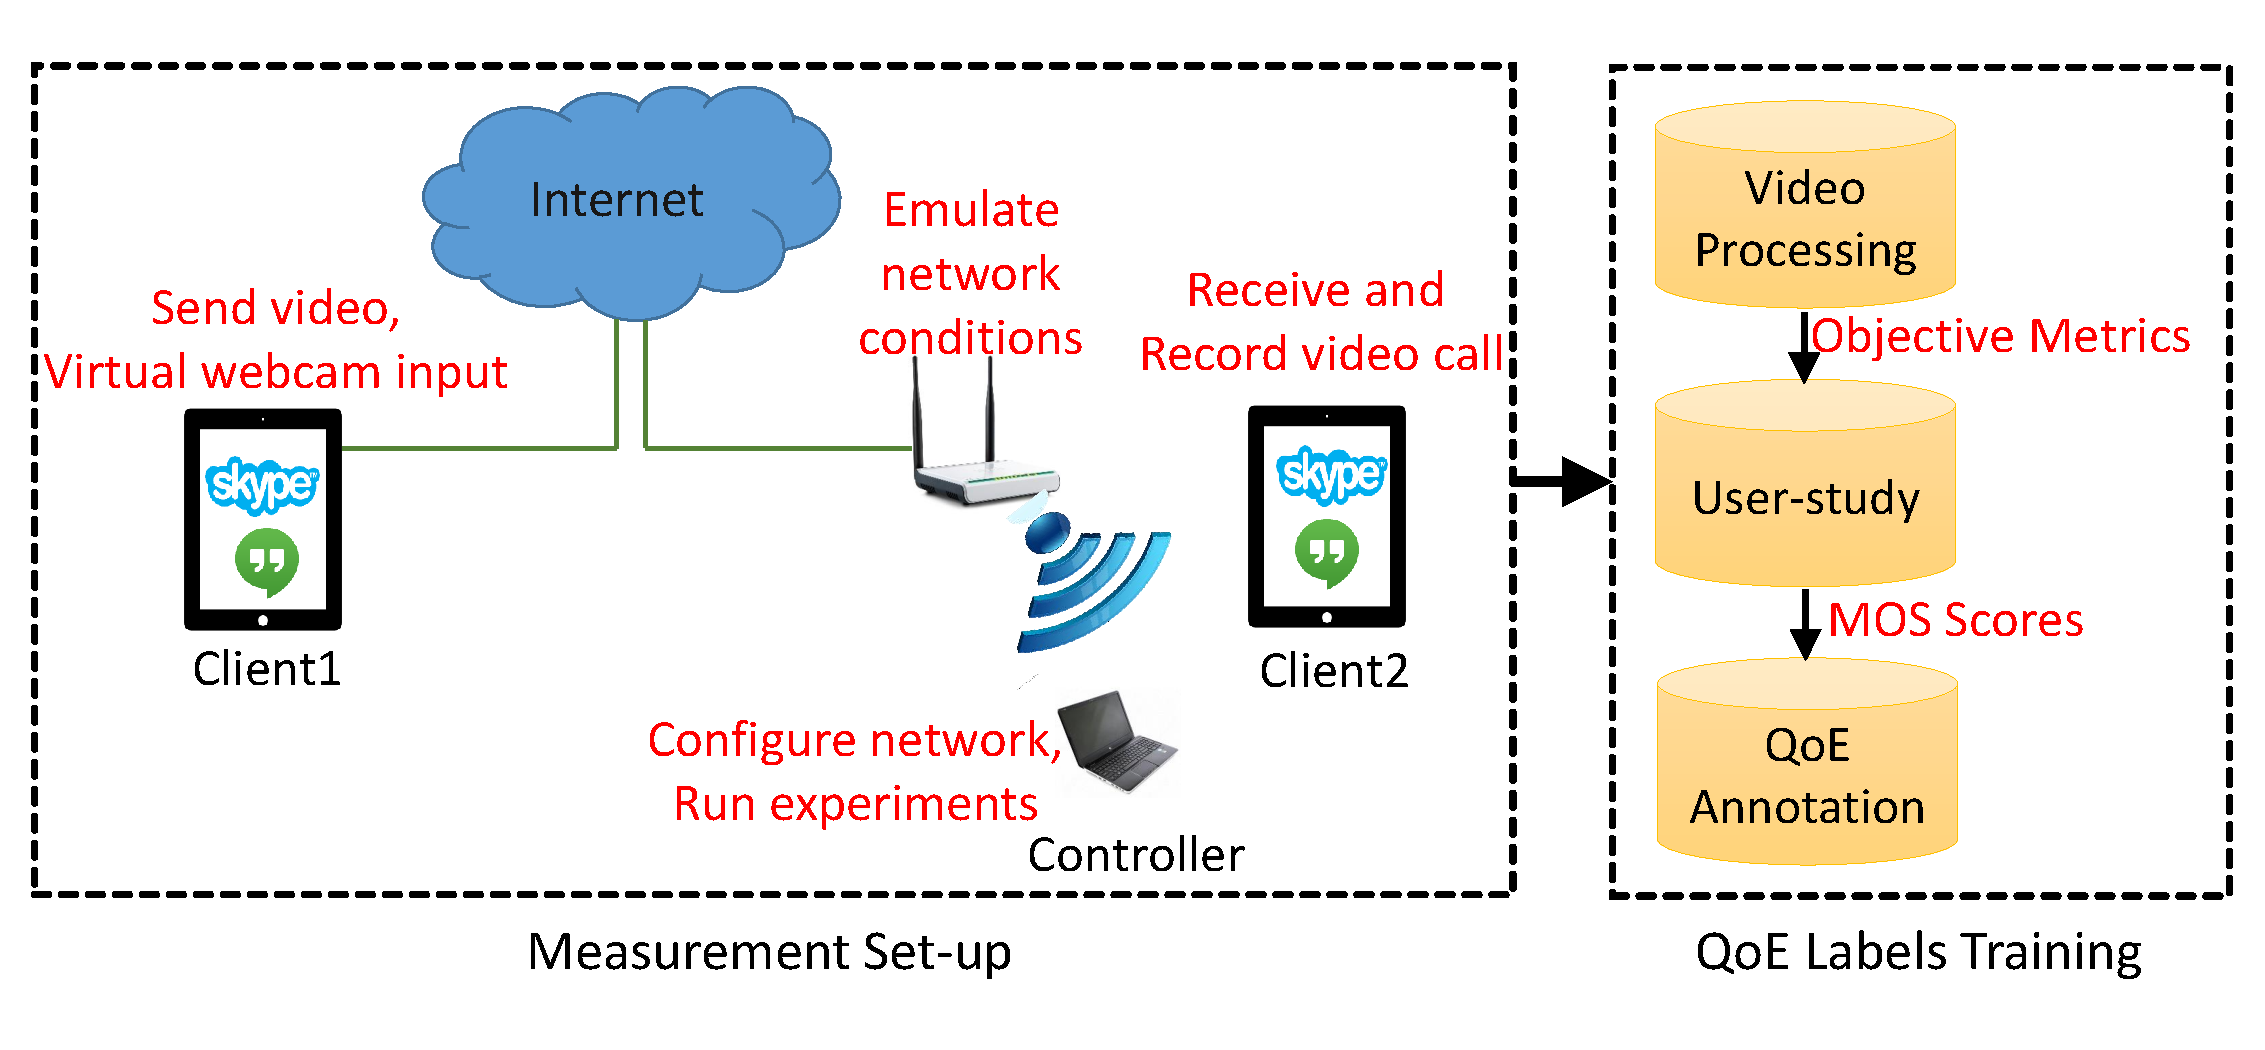
\includegraphics[width=\linewidth]{sections/network-work/setup}
     \vspace{-0.3in}
    \caption{Measurement set-up and system architecture. \textit{Left:} Video telephony measurements and recording video calls. \textit{Right:} Our framework processing recorded videos offline and extracting objective metrics to predict QoE labels.}
   \vspace{-0.2in}
  \label{fig:set-up}
\end{figure}
\begin{figure}[t]
  \centering
  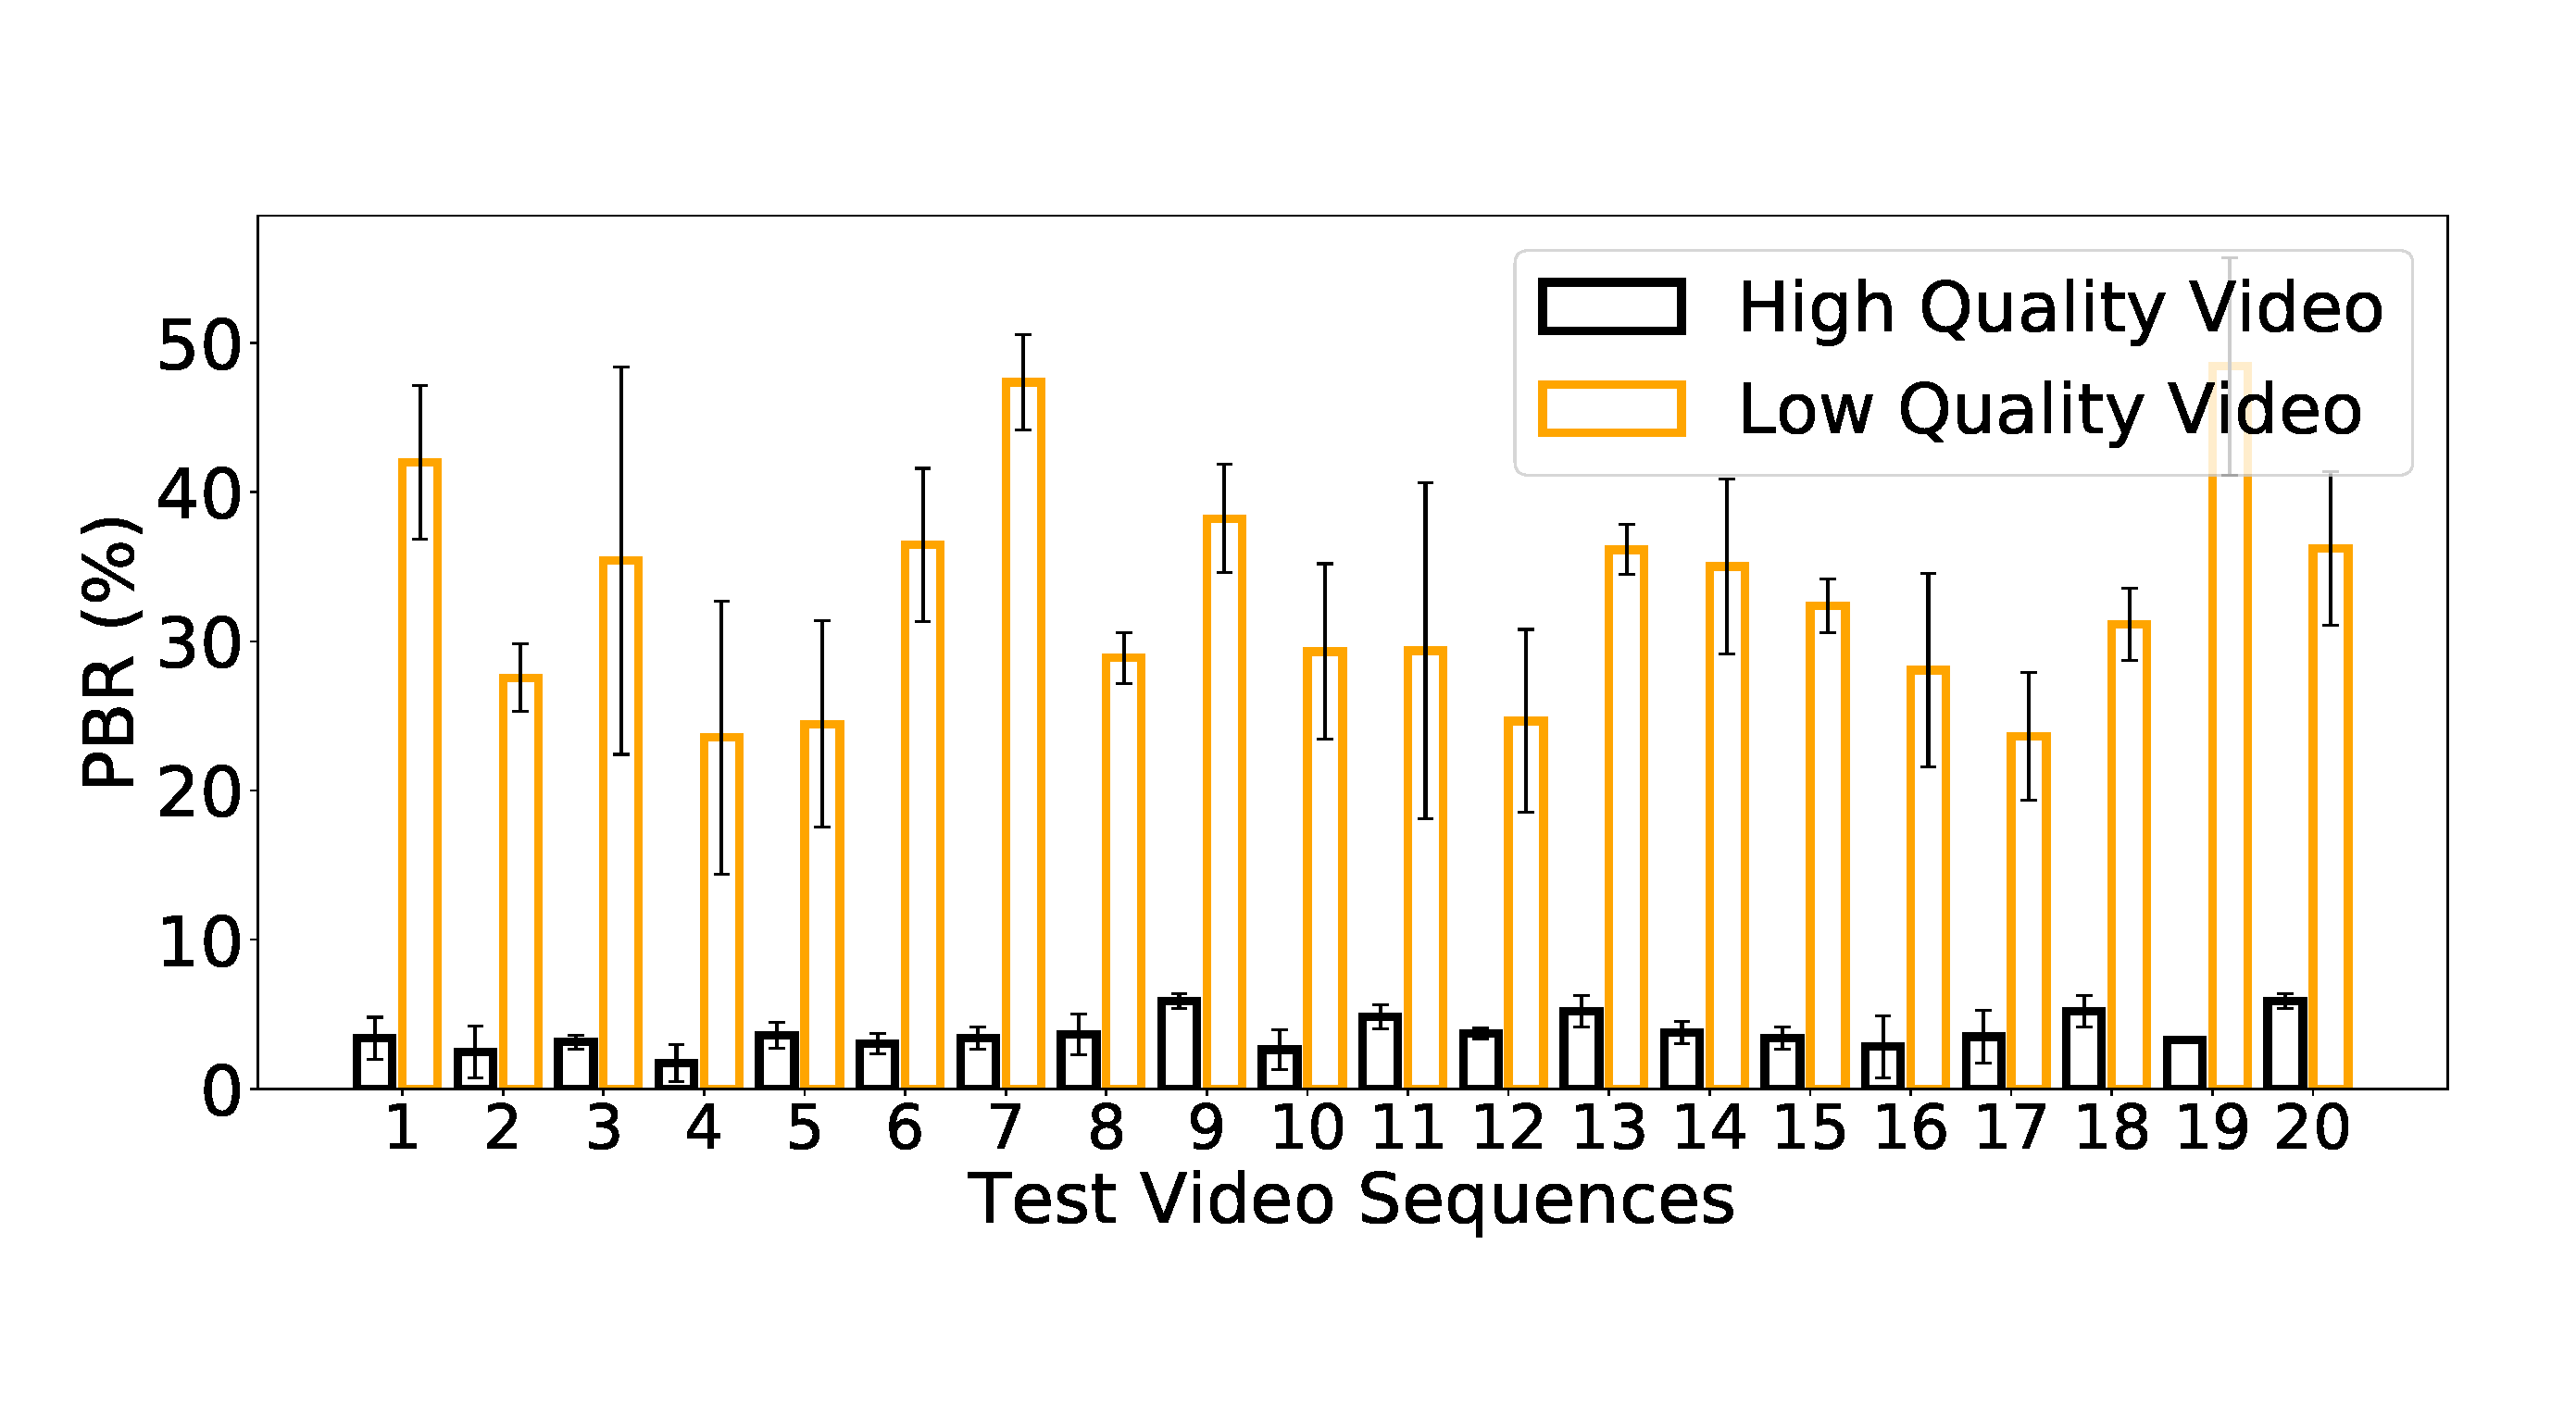
\includegraphics[width=\linewidth]{sections/network-work/bar-pbr}
   \vspace{-0.5in}
  \caption{Blur detection using PBR.}
\vspace{-2em}
  \label{fig:ourblurdetection}
\end{figure}

\subsection{Design for Scalable QoE Annotation} \label{label:design}
In this section, we first describe our framework and measurement methodology. 
We then explain our QoE metrics and evaluate them across different applications and devices. We validate that our metrics capture video artefacts caused by diverse network conditions.
\subsubsection{Measurement Methodology}

\noindent \textbf{Set-up:} 
In Figure~\ref{fig:set-up}, we show our measurement set-up and QoE labeling framework. 
Since video telephony is an interactive application, it requires at least two participating network end-points (clients). In our set-up, we use a mobile device on our local enterprise WiFi network (Client 1) and an Amazon-provided instance as the second end-point (Client 2). Both clients can run Skype or Hangouts\footnote{For FaceTime, we use 2 local clients (iPhone/iPad and MacBook Air) on different sub-networks, as creating virtual iOS and web-cam is challenging.}. 
When the video call is placed from Client 1 to Client 2, Client 2 runs a virtual web-cam that inputs a video file in telephony application instead of camera feed; at Client 1, the video is received during the call.
At the Amazon Client 2, we use \textit{manycam} \cite{mancam}, a virtual web-cam tool. 
This tool can be used with multiple video applications in parallel for automation. 
In our LAN, a controller sits  to emulate diverse network conditions and to run experiments on the connected mobile device  through Android debug bridge (ADB) interface (via USB or WiFi connection). 
To automate the video call process, we use AndroidViewClient (AVC) library \cite{awc}.
Once the received call is accepted, we start the screen recording of the video call session.   The videos are recorded using Az screen recorder \cite{azscreen}. 
The recorded videos are sent to video processing module to calculate the objective QoE metrics. 
We use Ffmpeg \cite{ffmpeg} tool to extract our QoE metrics. Ffmpeg is a video framework with large collection of coding libraries. To validate our metrics and translate them into user experience, the videos are then shown to users to rate their experience. 
Finally, we retrieve MOS from all users and map our QoE metrics to MOS. We delve into the details of our user  study and modeling in Section~\ref{label:results}.
%We use Ffmpeg to convert, encode and manipulate videos to extract Rbitrate, RFps and freeze ratio etc. 
%We use Matlab and OpenCV to convert video to images and extract blur metric of individual images.

%\begin{table}[t]
%  \centering
%    \scalebox{1.08}{
%  \begin{tabular}{c|c|c|c|c}
%  \hline \hline
%    \textbf{Video Sequence} & \textbf{Frames} & \textbf{Fps} & \textbf{bitrate (Kbps)} & \textbf{Motion} \\
%    \hline
%    \hline
%     $TalkShow.y4m$ & 600 & 40 & 1360 & low \\ \hline
%     $Bunny.y4m$ & 504 & 25 & 3500 & average \\ \hline
%     $Bus.y4m$ & 500 & 12 & 19037 & high \\ \hline
%  \end{tabular}
%    }
%  \caption{Motion classification based on Video Coding Parameters and Corresponding QoE Ground-truth}
%  \label{tab:table2}
%\end{table}

\begin{figure*}
%    \centering
%    \vspace*{-1em}
%    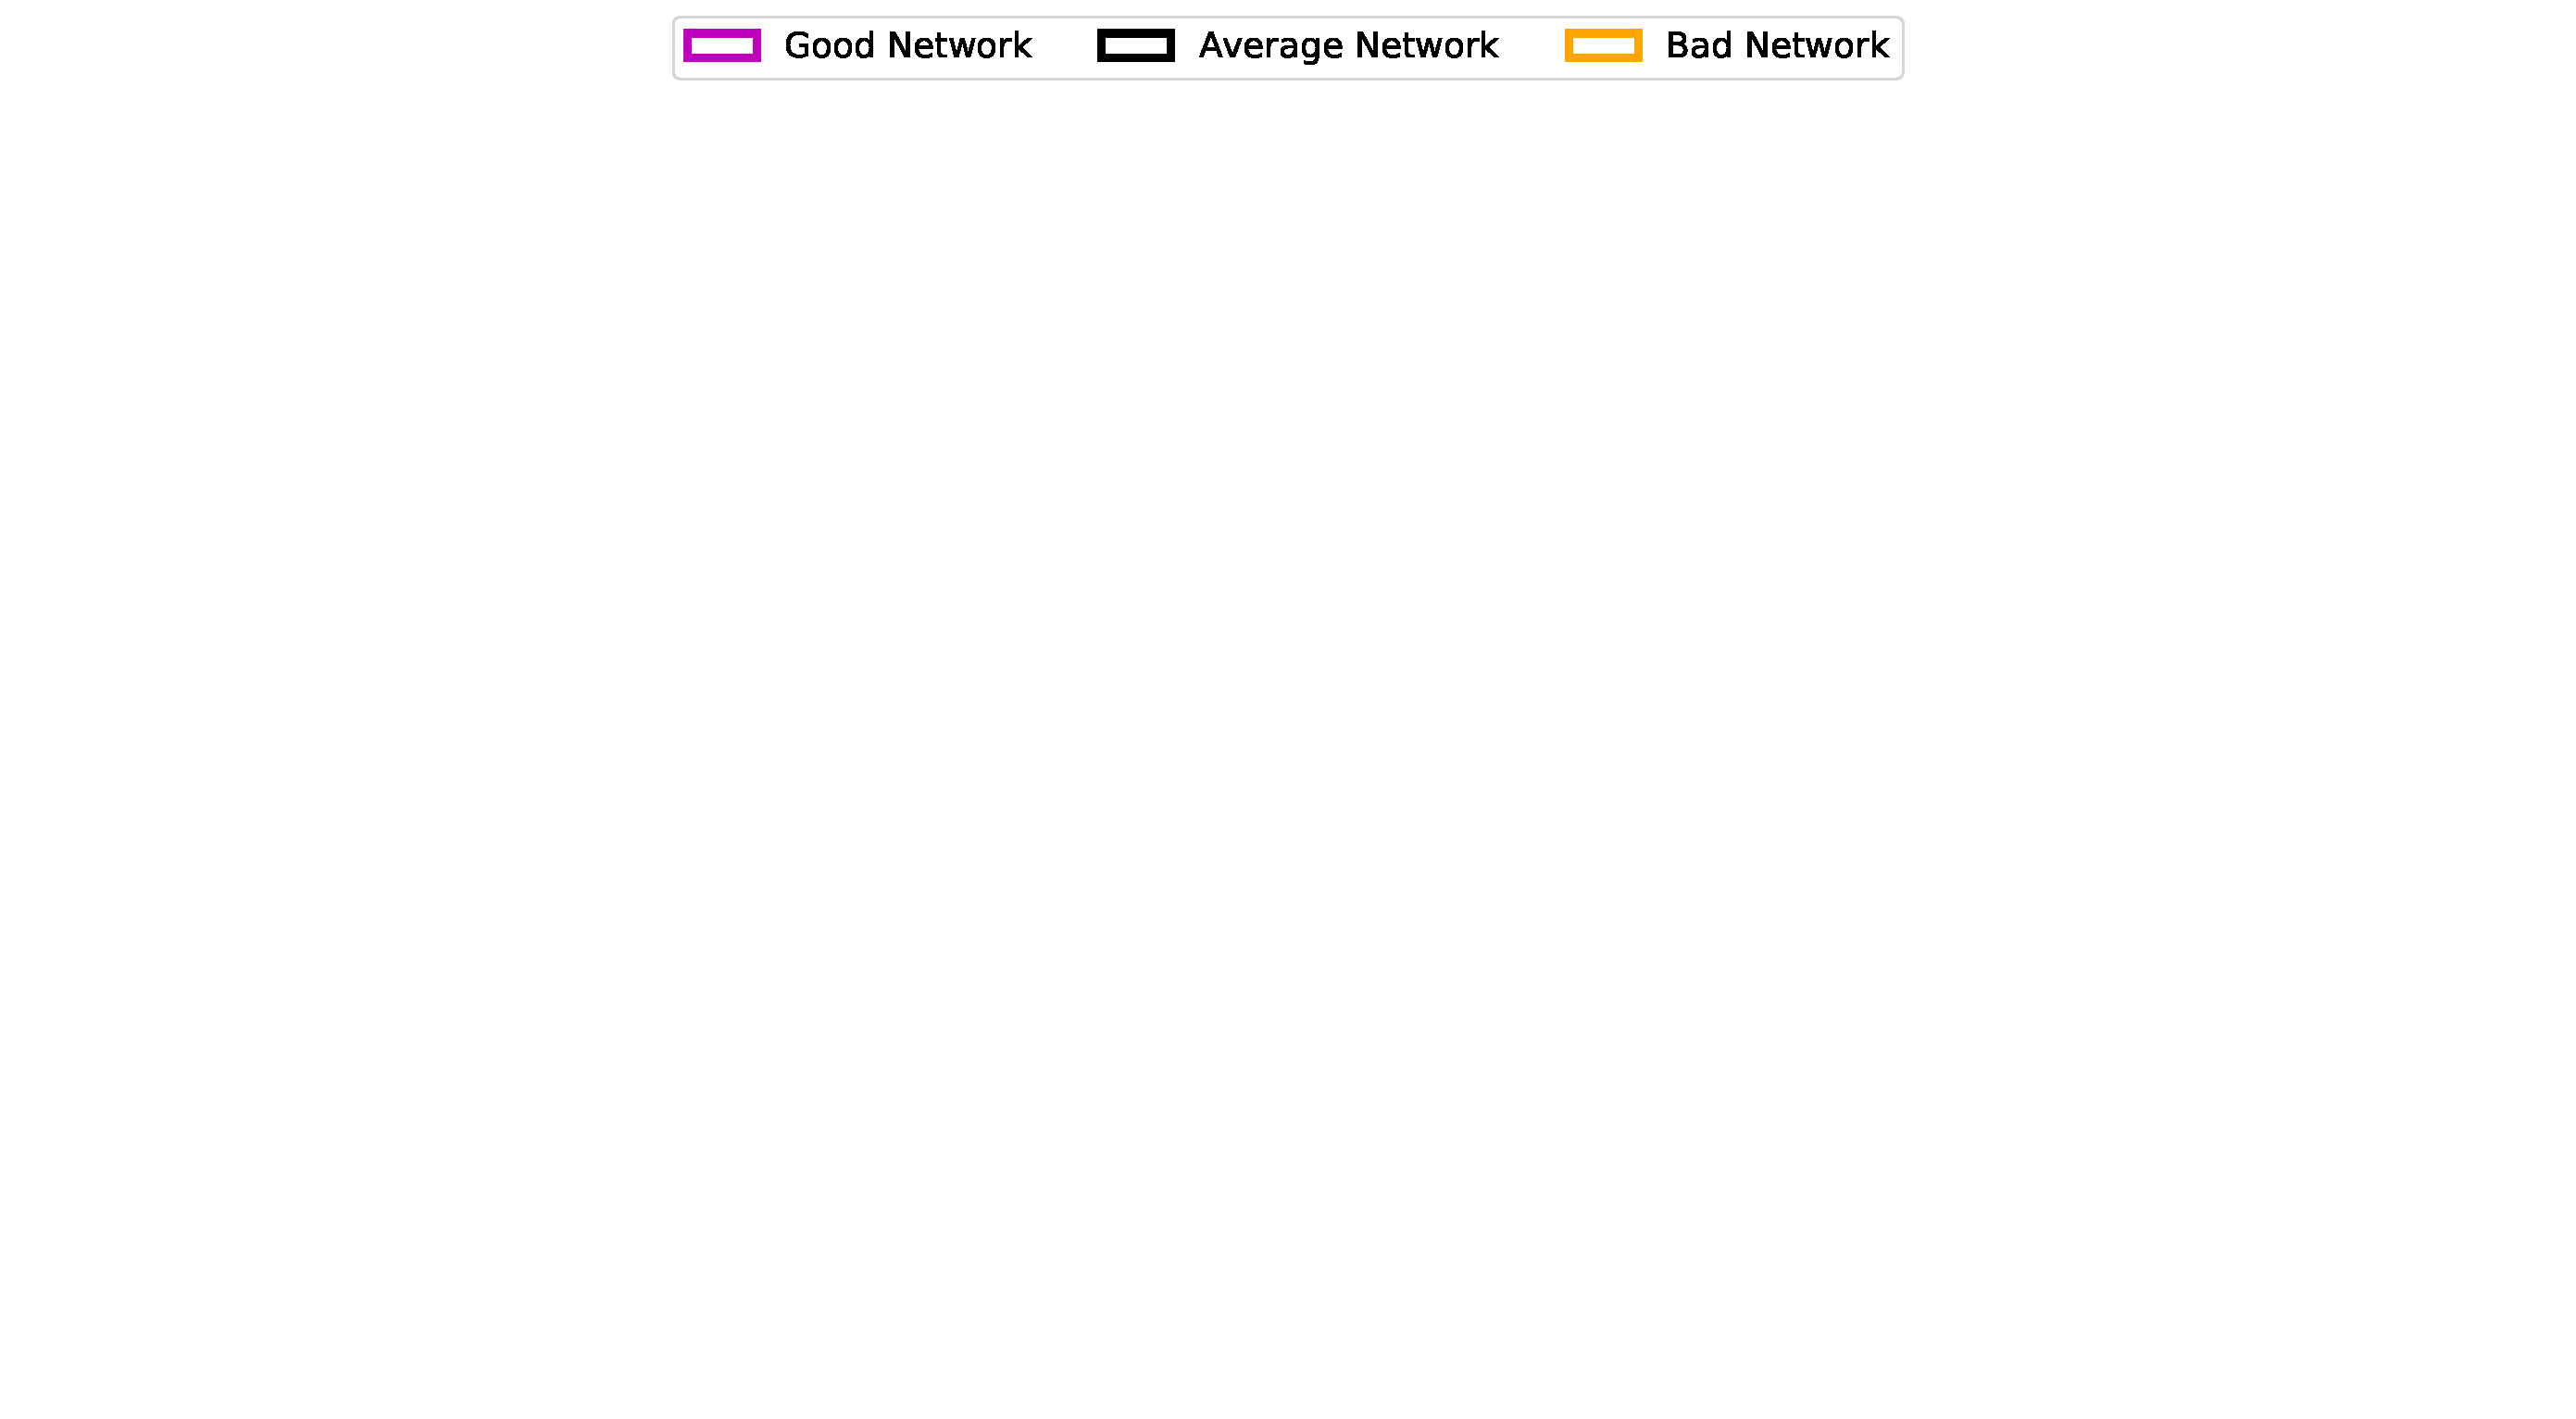
\includegraphics[trim={2.5cm 24.5cm 2.5cm 0},clip,width=0.8\linewidth]{sections/network-work/legend4.pdf}
%  \subfigure[Content and Motion]{\hspace*{-1em}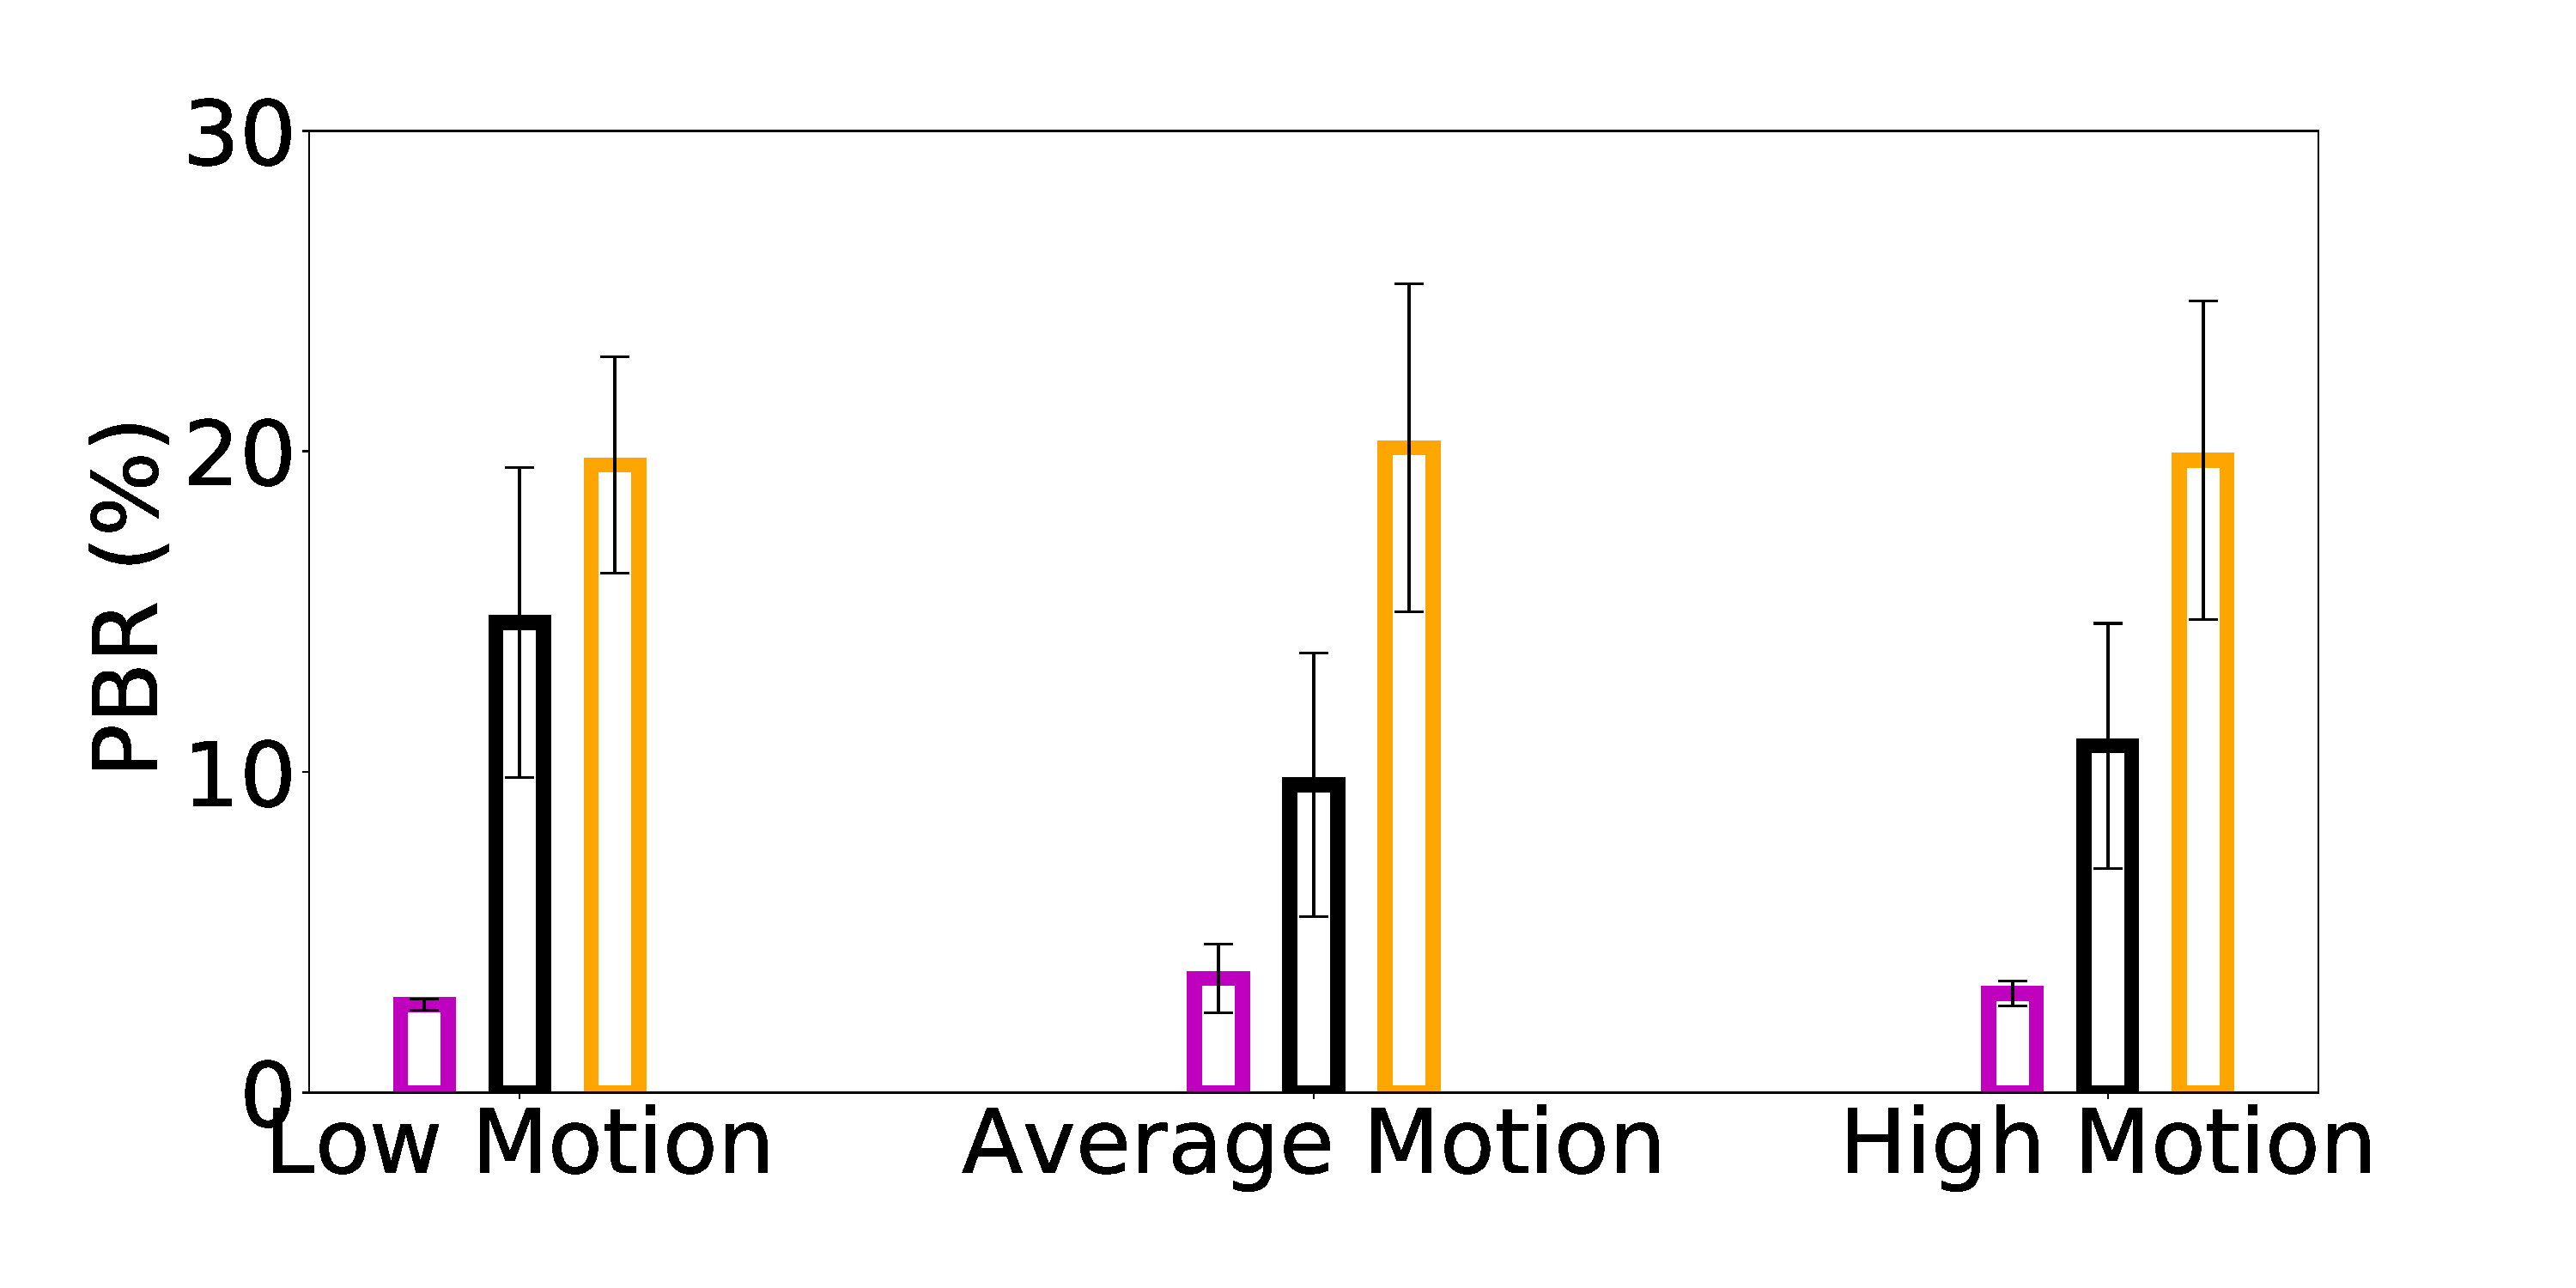
\includegraphics[width=0.33\textwidth]{sections/network-work/content-bitrate}\label{fig:cont-pbr} \vspace*{-3em}}~
%  \subfigure[Applications]{\hspace*{-1em}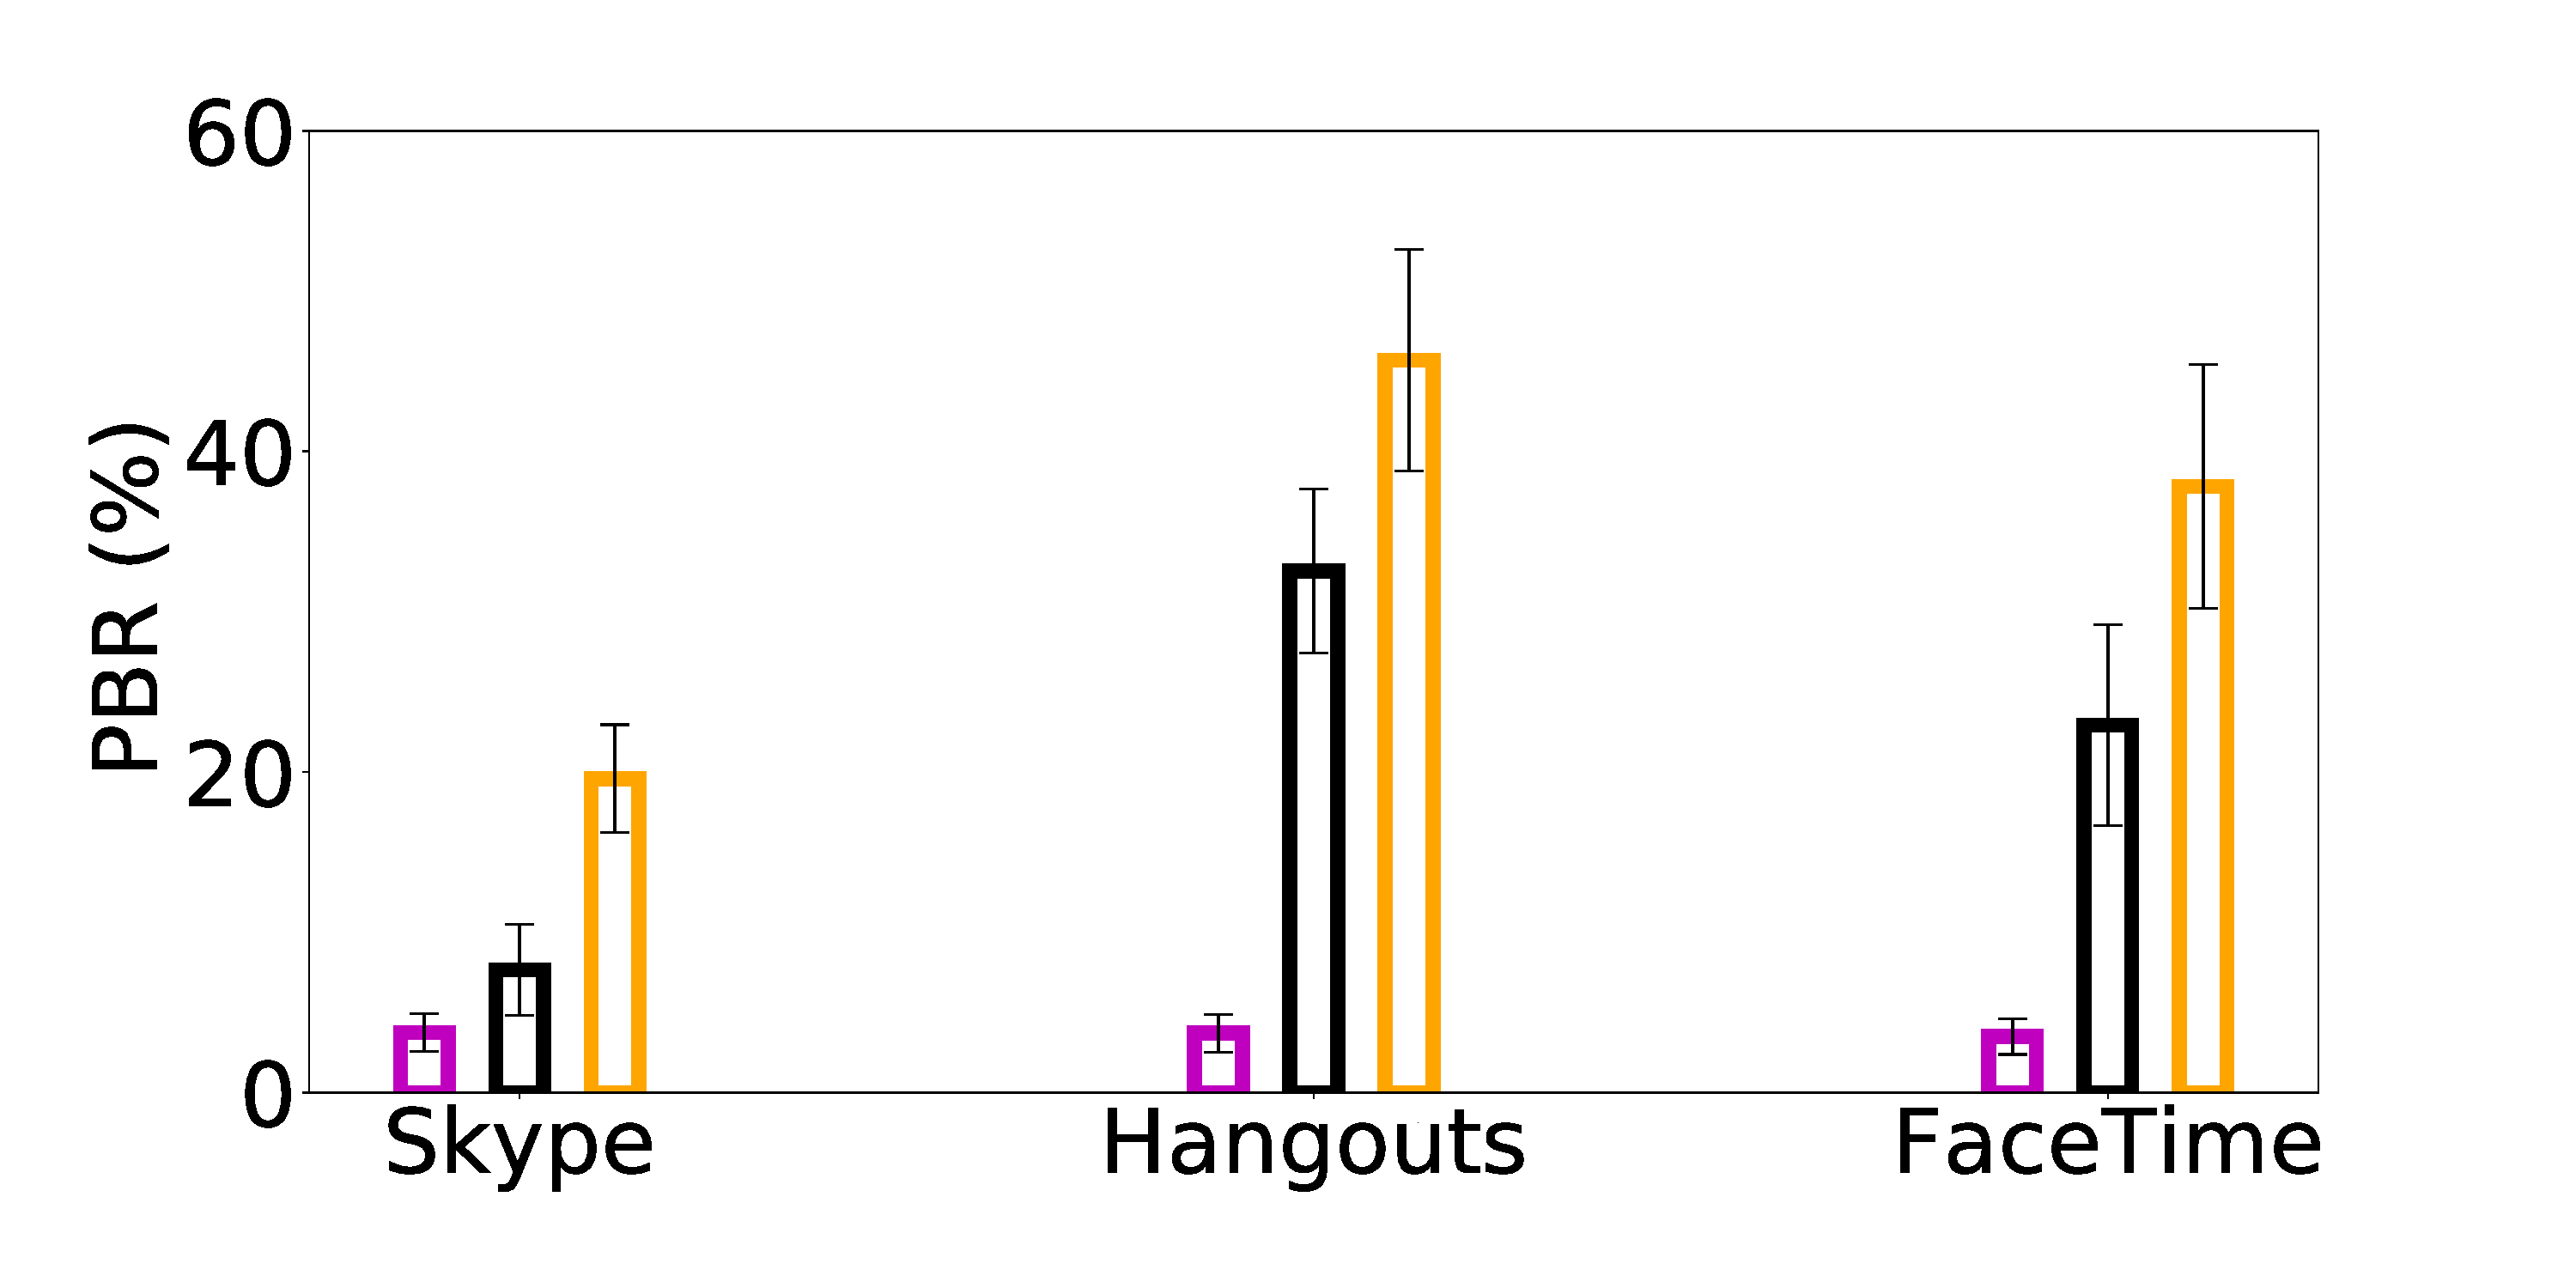
\includegraphics[width=0.33\textwidth]{sections/network-work/app-bitrate}\label{fig:app-pbr} \vspace*{-3em}}~
%   \subfigure[Devices] {\hspace*{-1em} 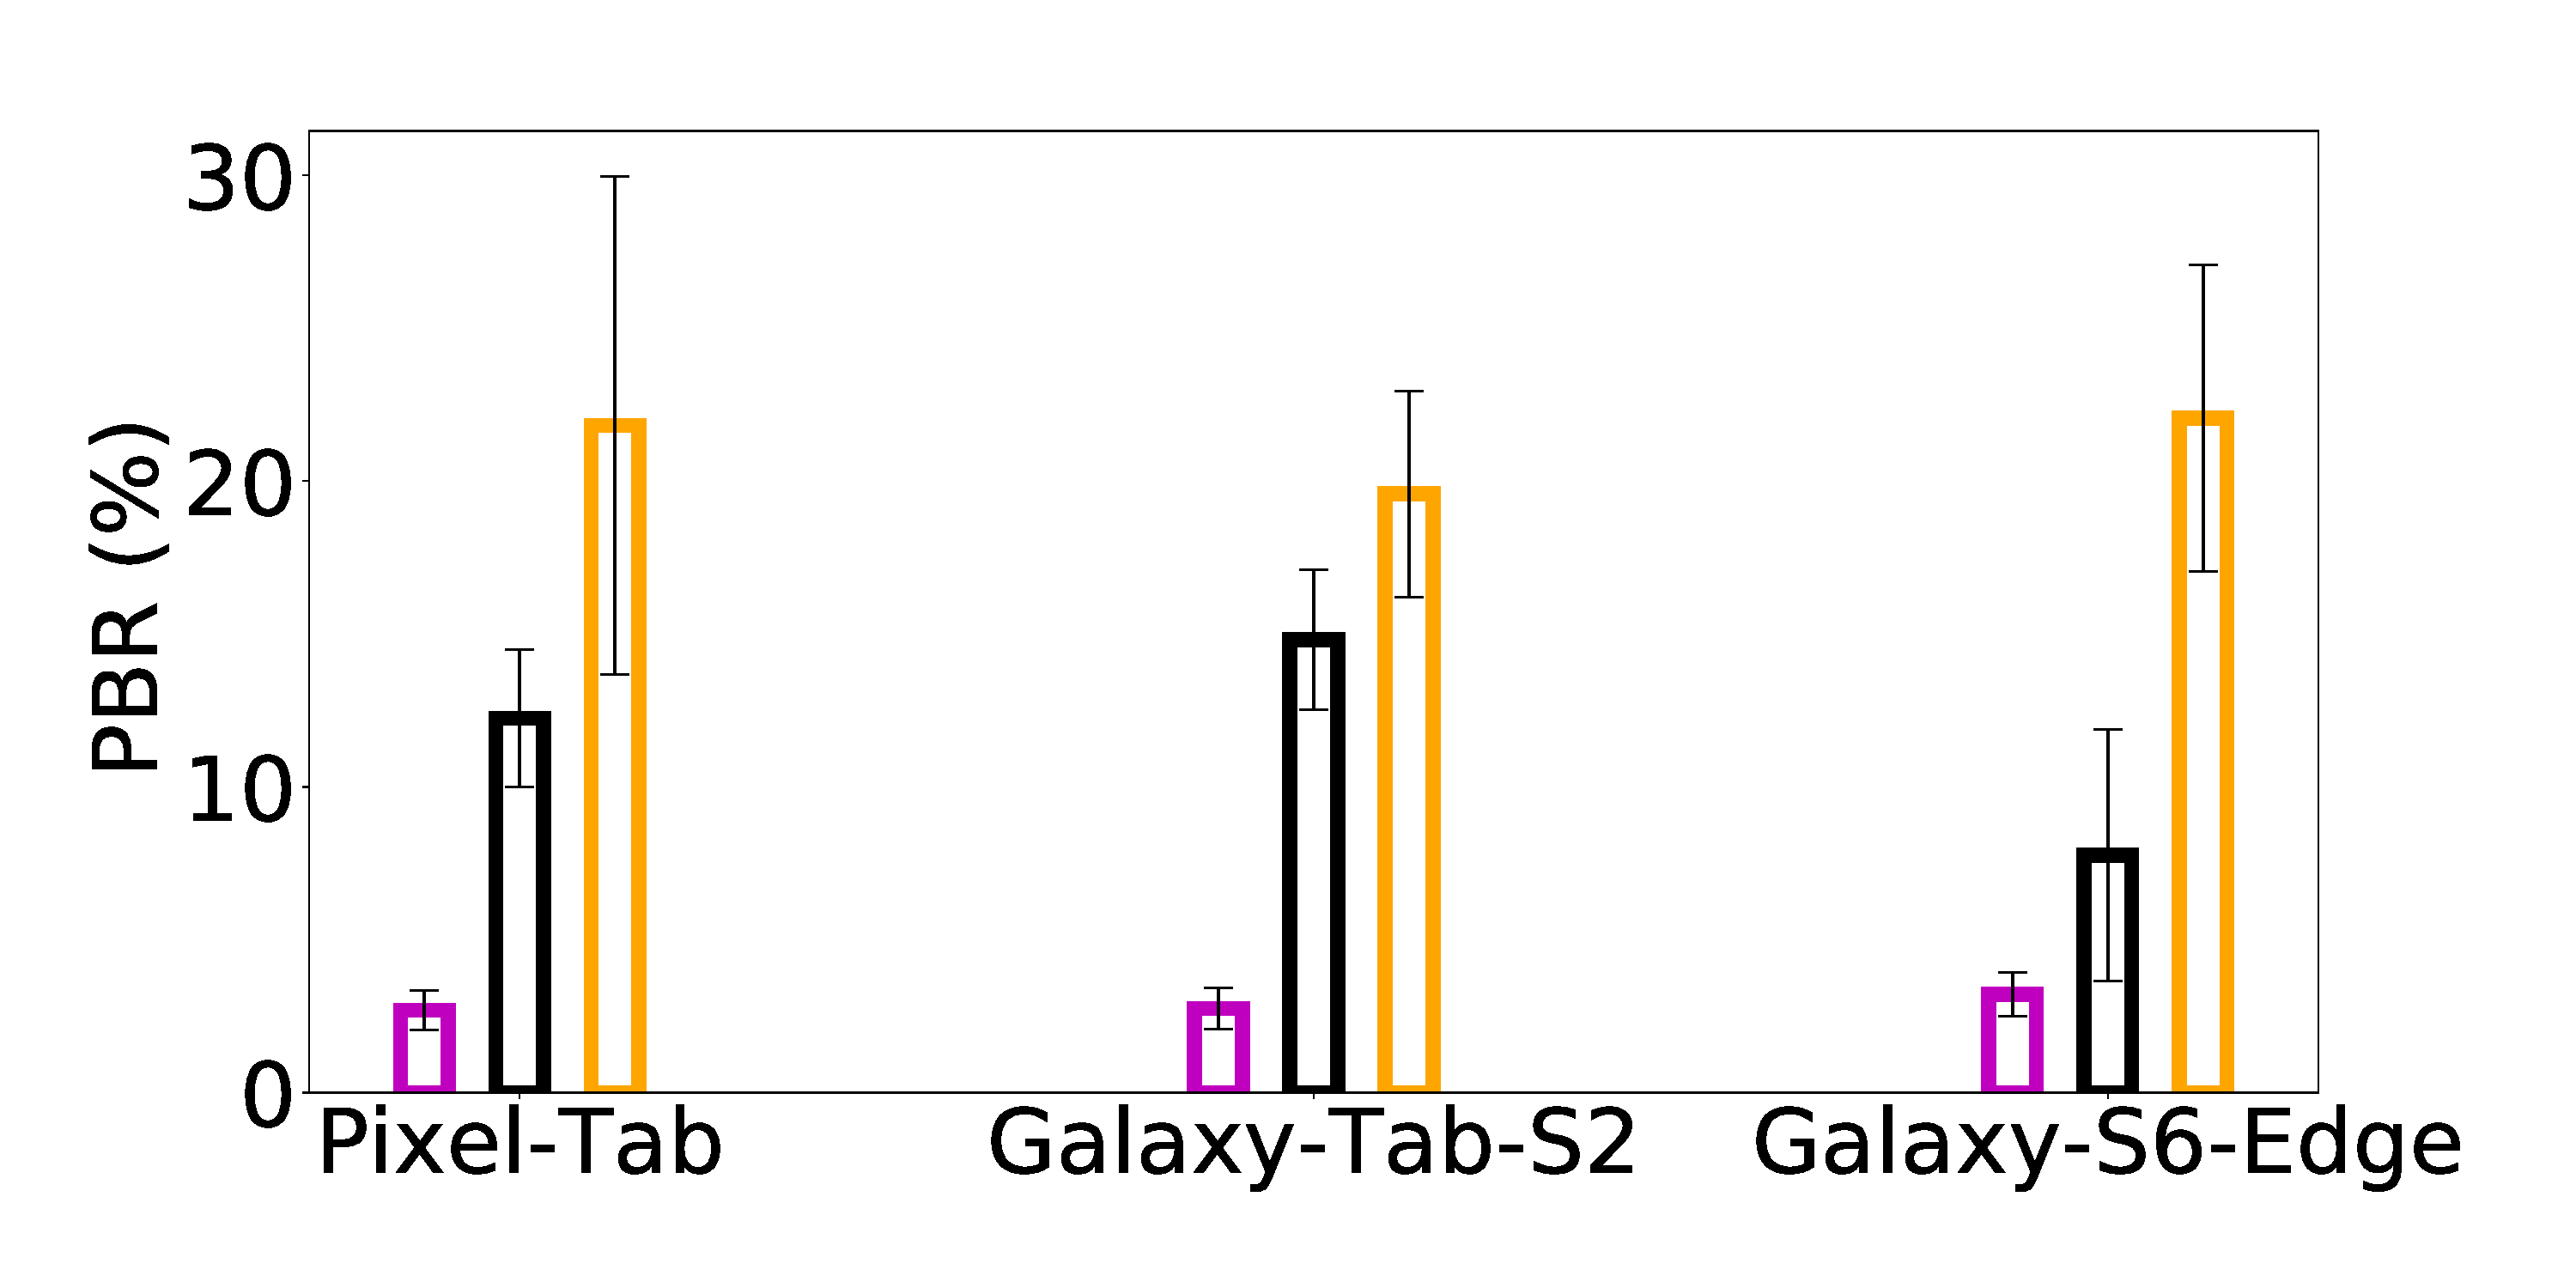
\includegraphics[width=0.33\textwidth]{sections/network-work/dev-bitrate}\label{fig:dev-pbr} \vspace*{-3em}}
%     \subfigure[Content and Motion]{\hspace*{-1em}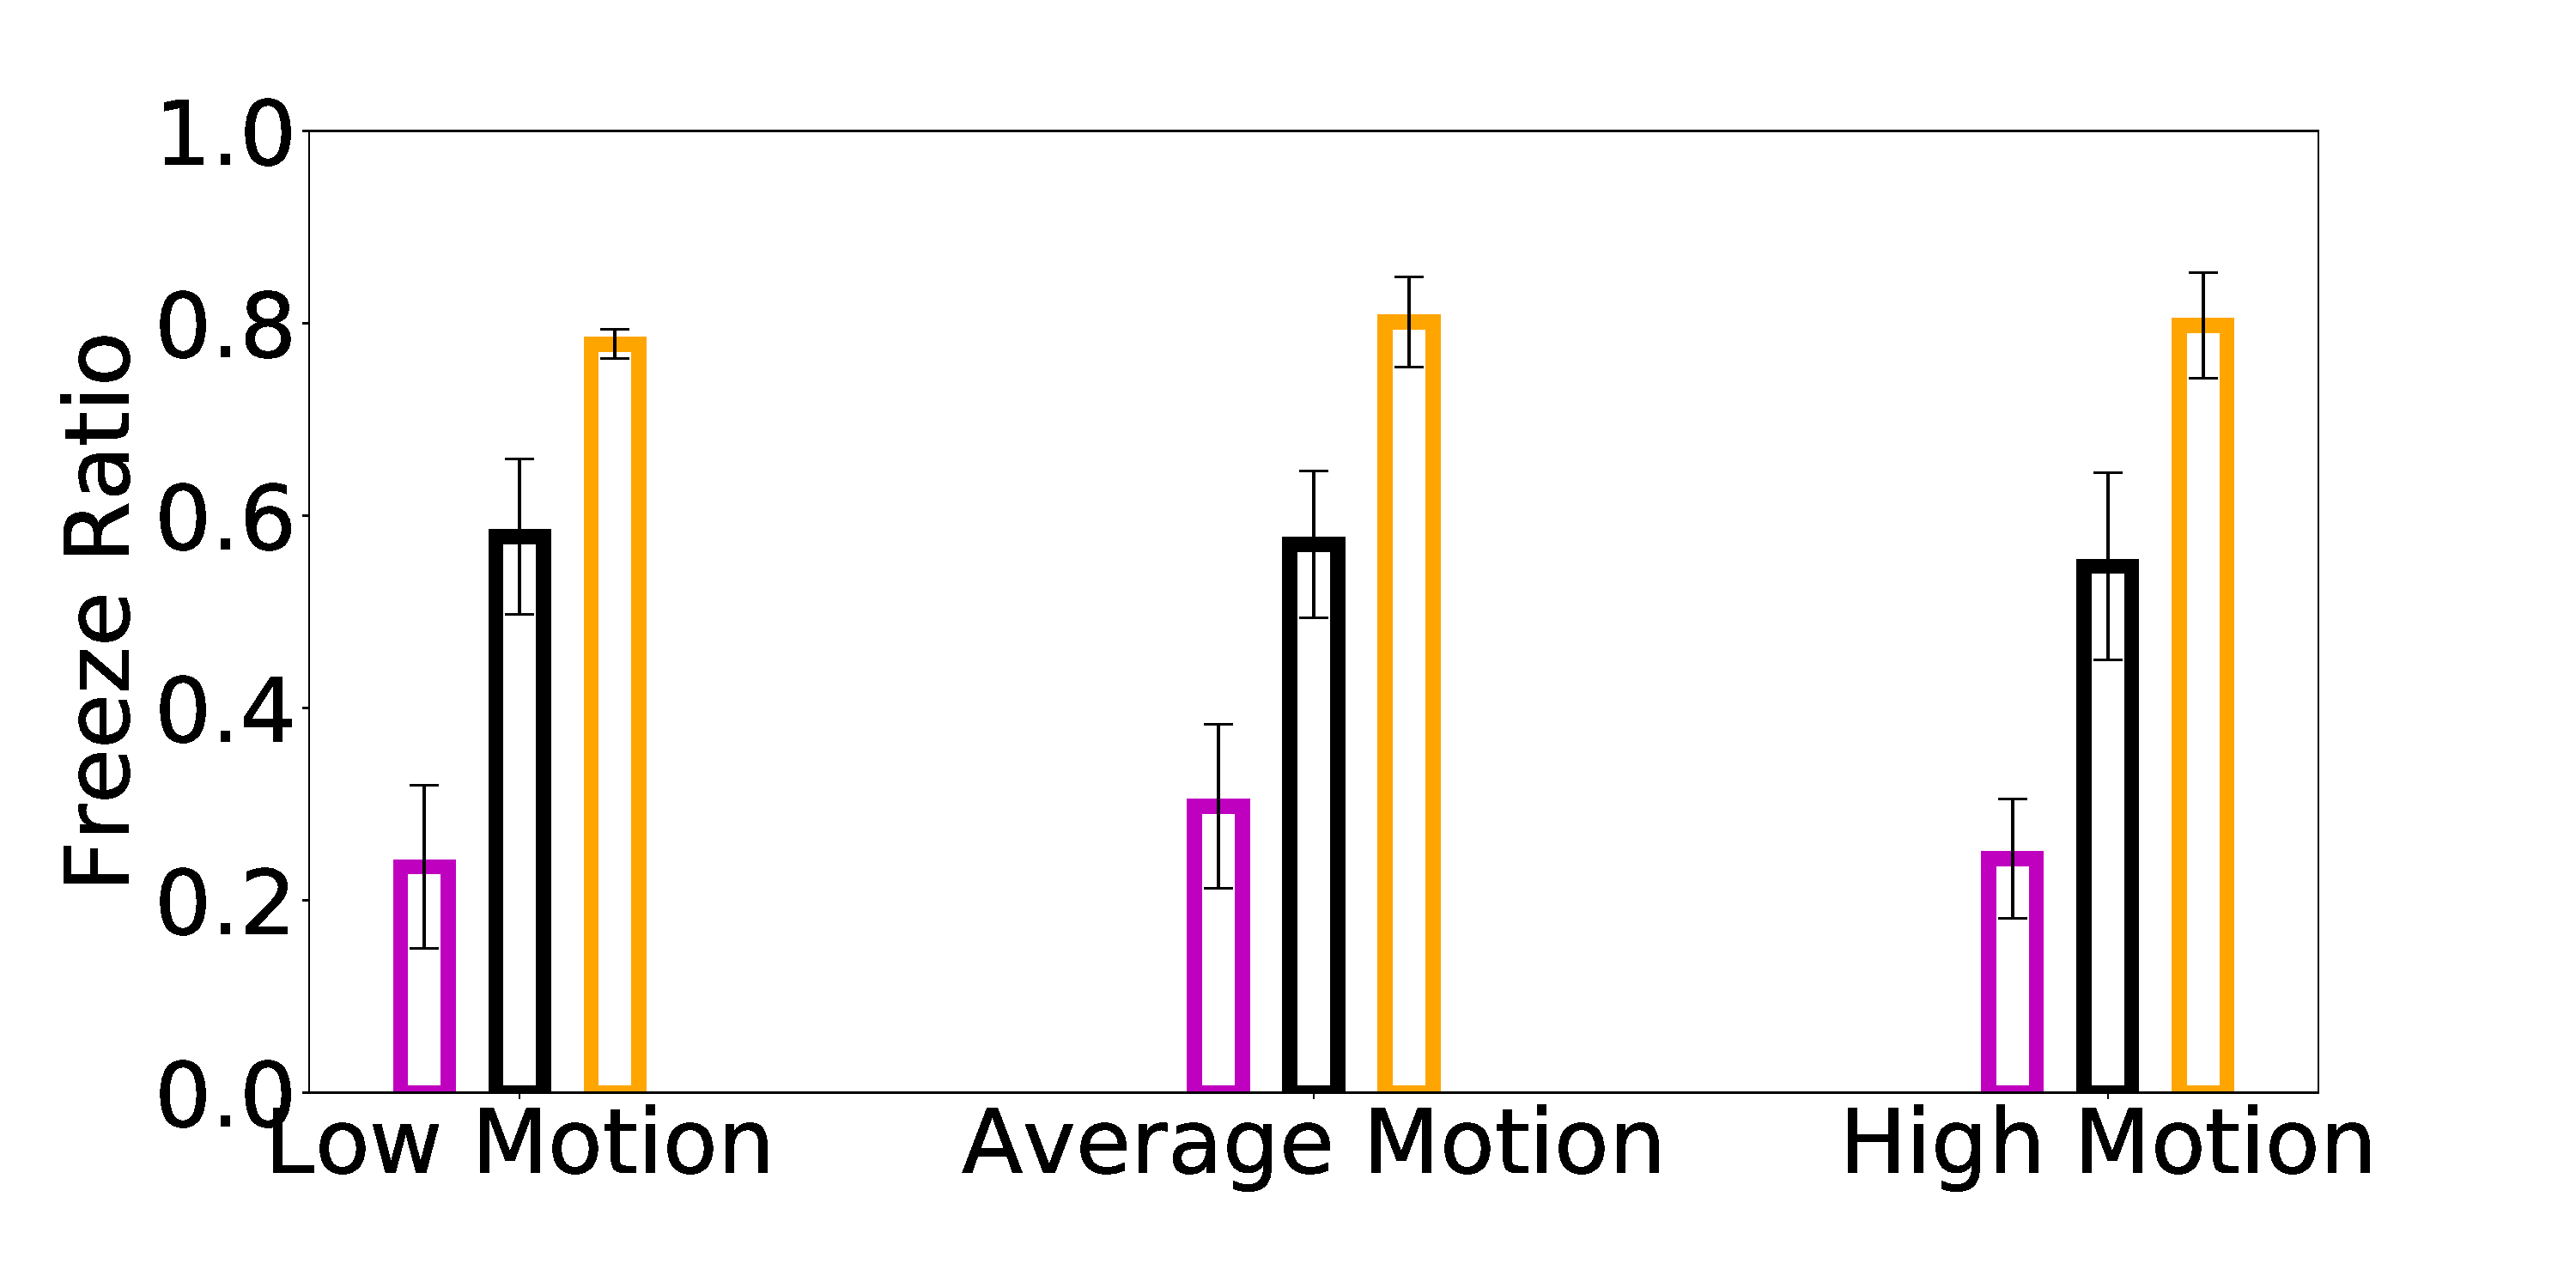
\includegraphics[width=0.33\textwidth]{sections/network-work/content-stutter}\label{fig:cont-st}}~
%     \subfigure[Applications]{\hspace*{-1em}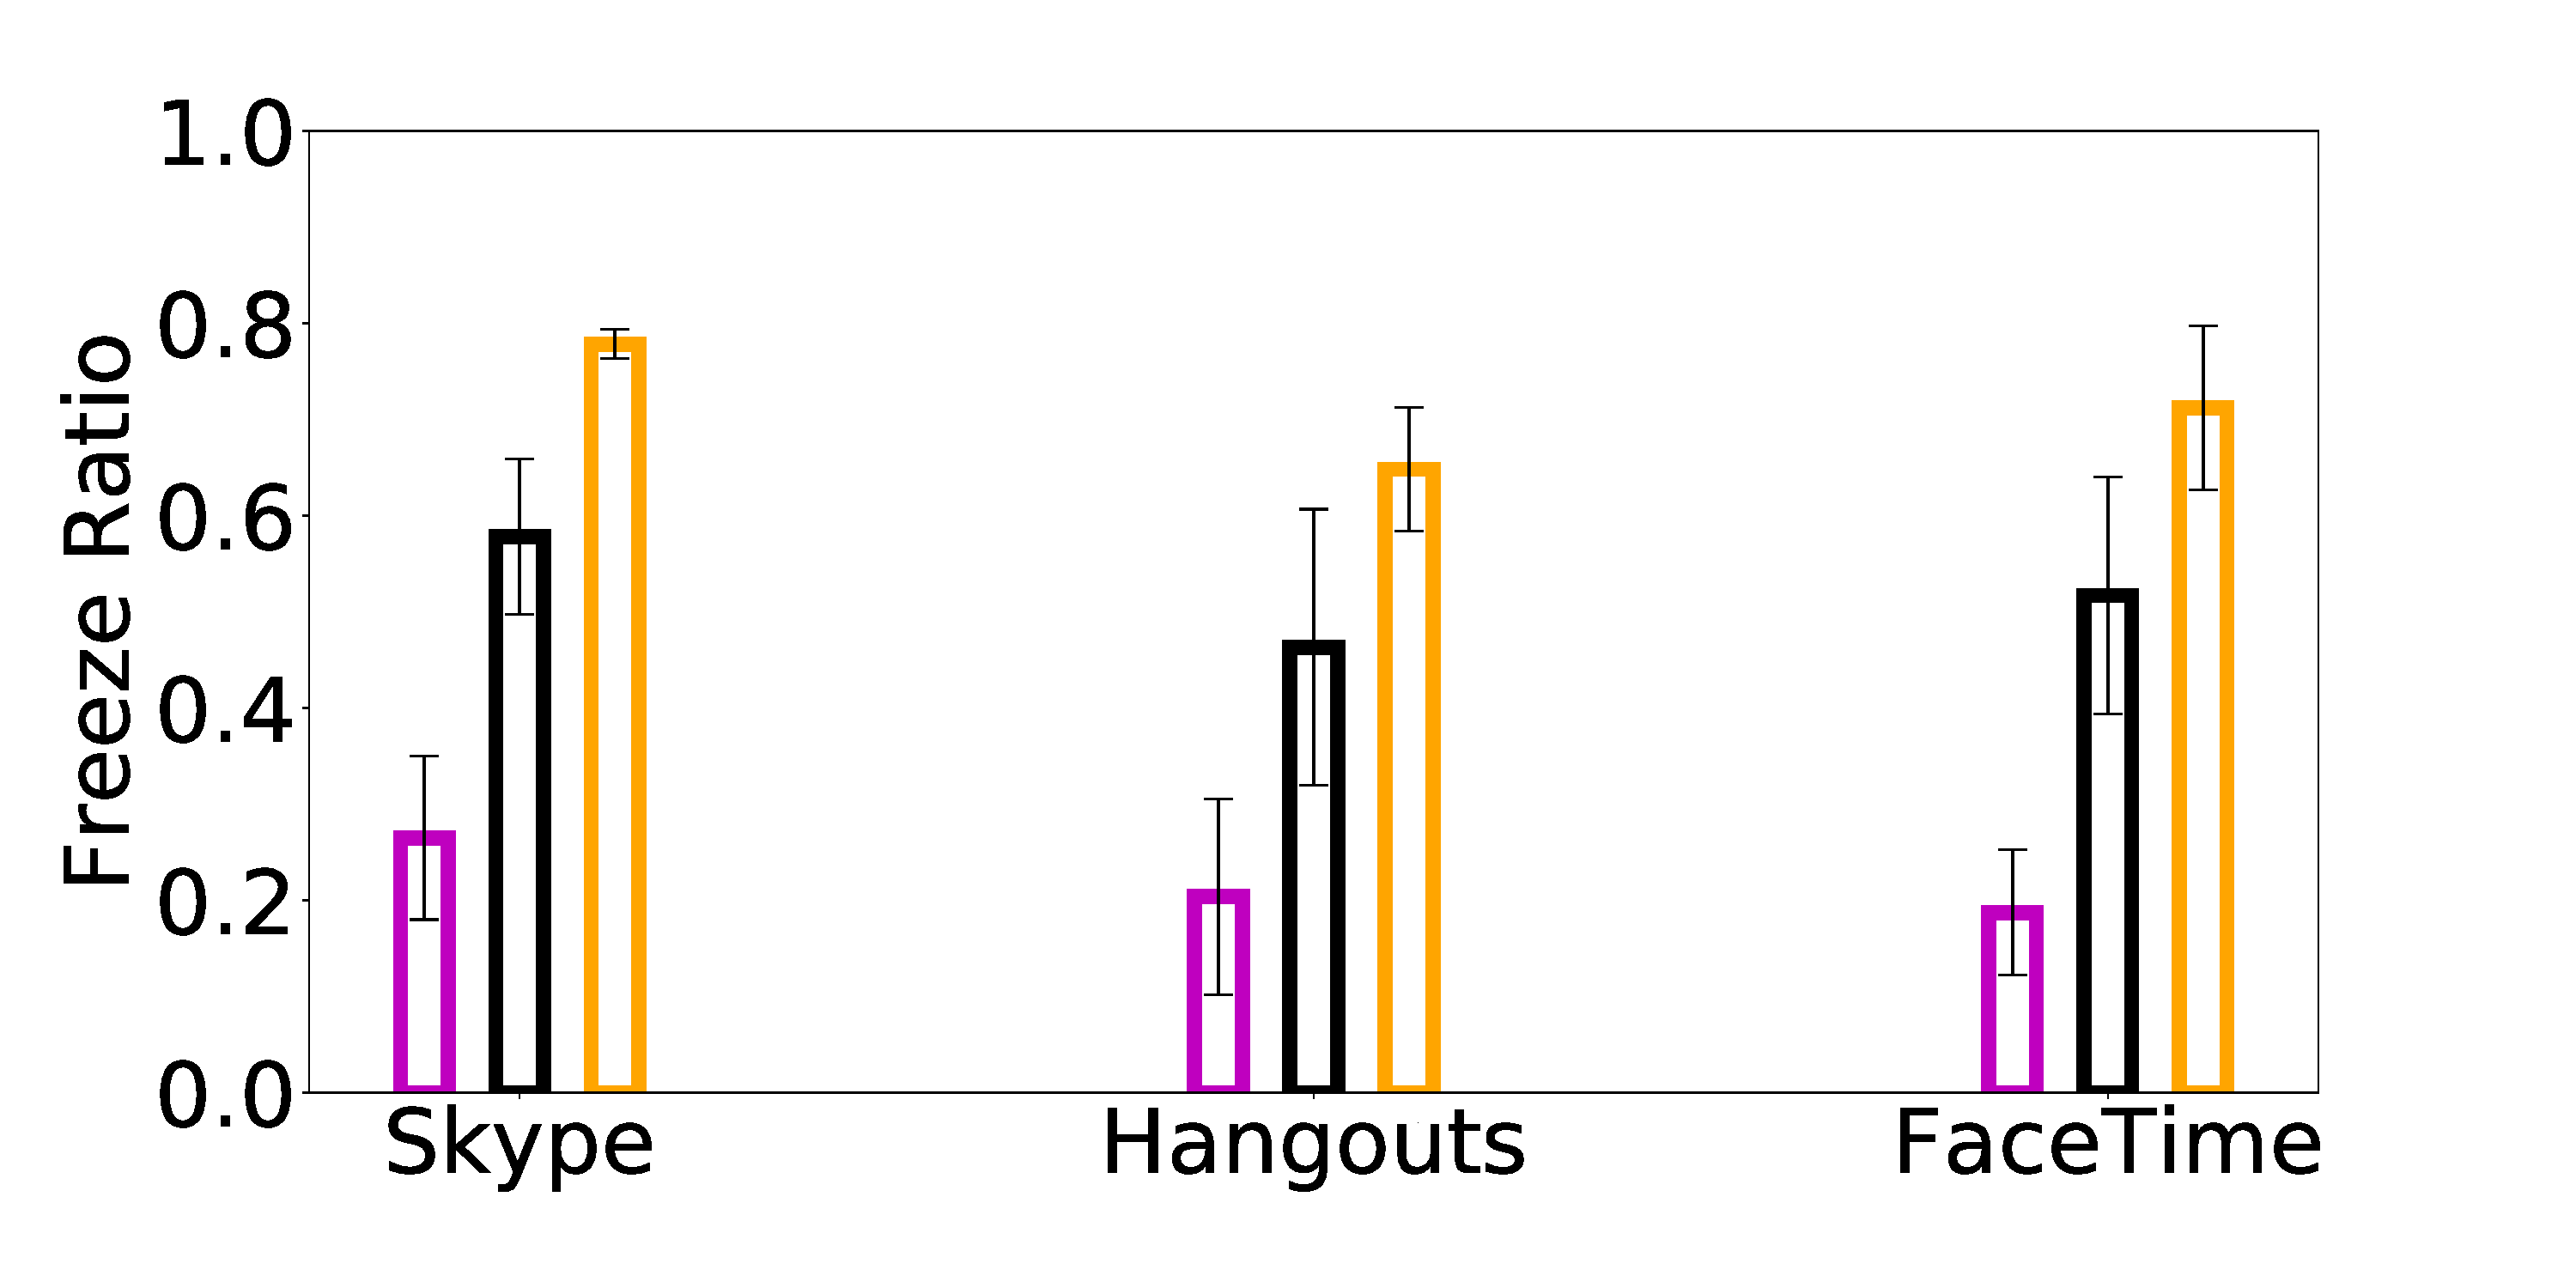
\includegraphics[width=0.33\textwidth]{sections/network-work/app-stutter}\label{fig:app-st}}~
%     \subfigure[Devices] {\hspace*{-1em} 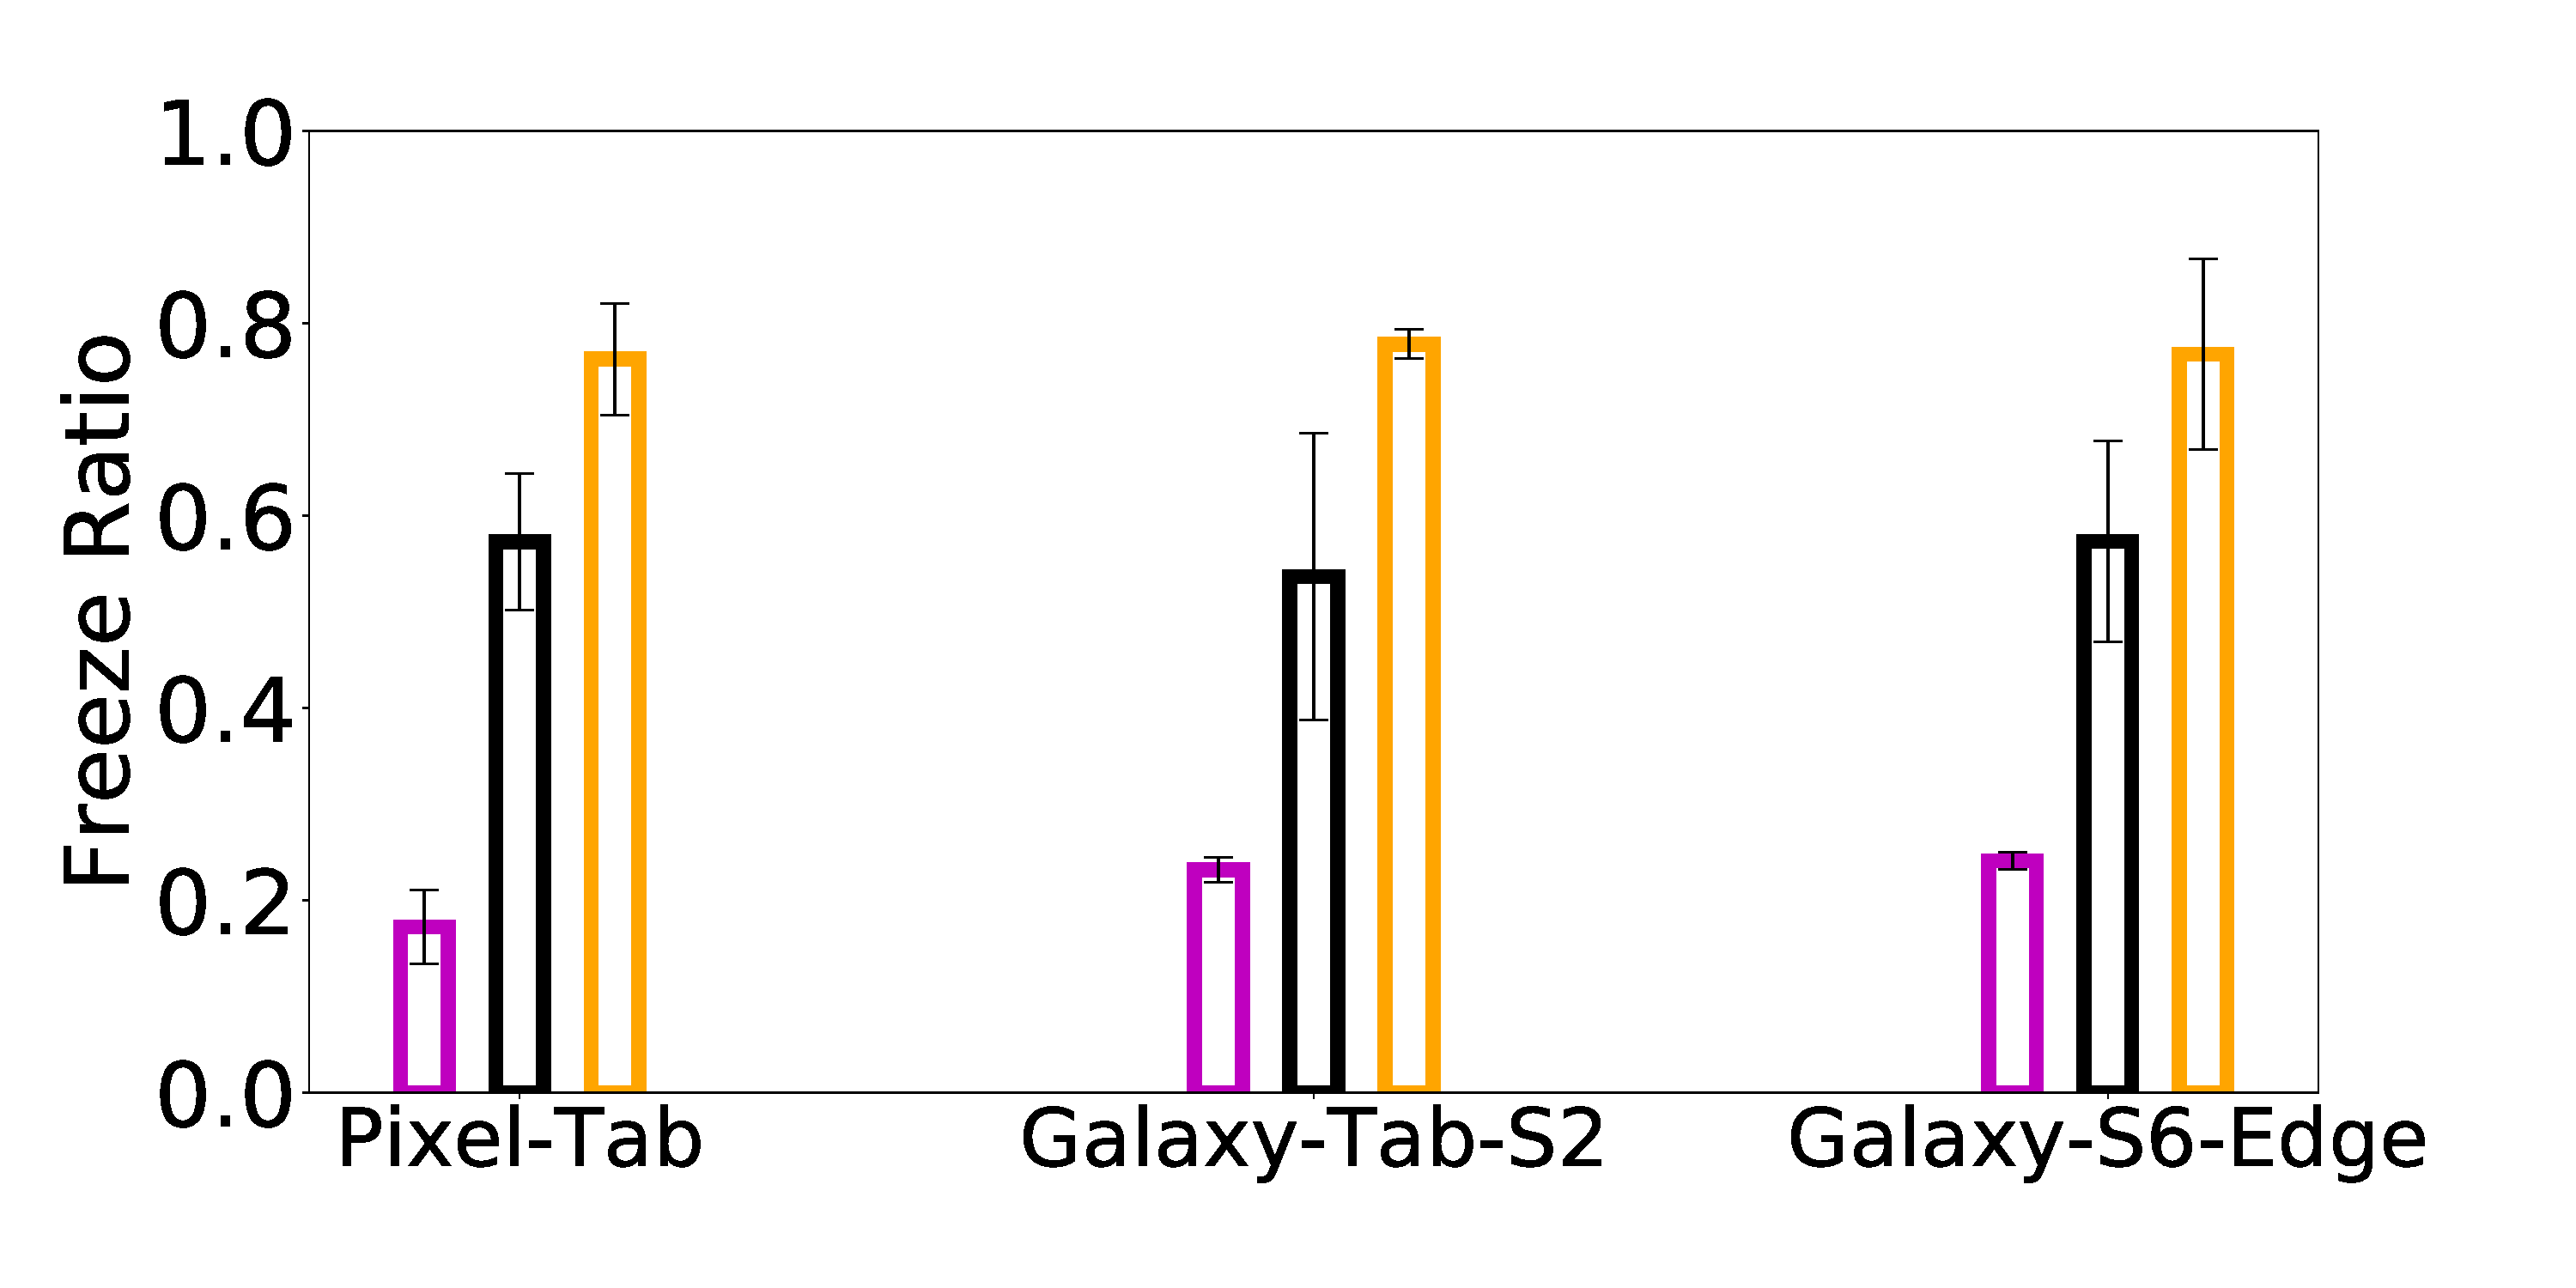
\includegraphics[width=0.33\textwidth]{sections/network-work/dev-stutter} \label{fig:dev-st}}
    \begin{subfigure}[b]{0.33\textwidth}
        \centering
        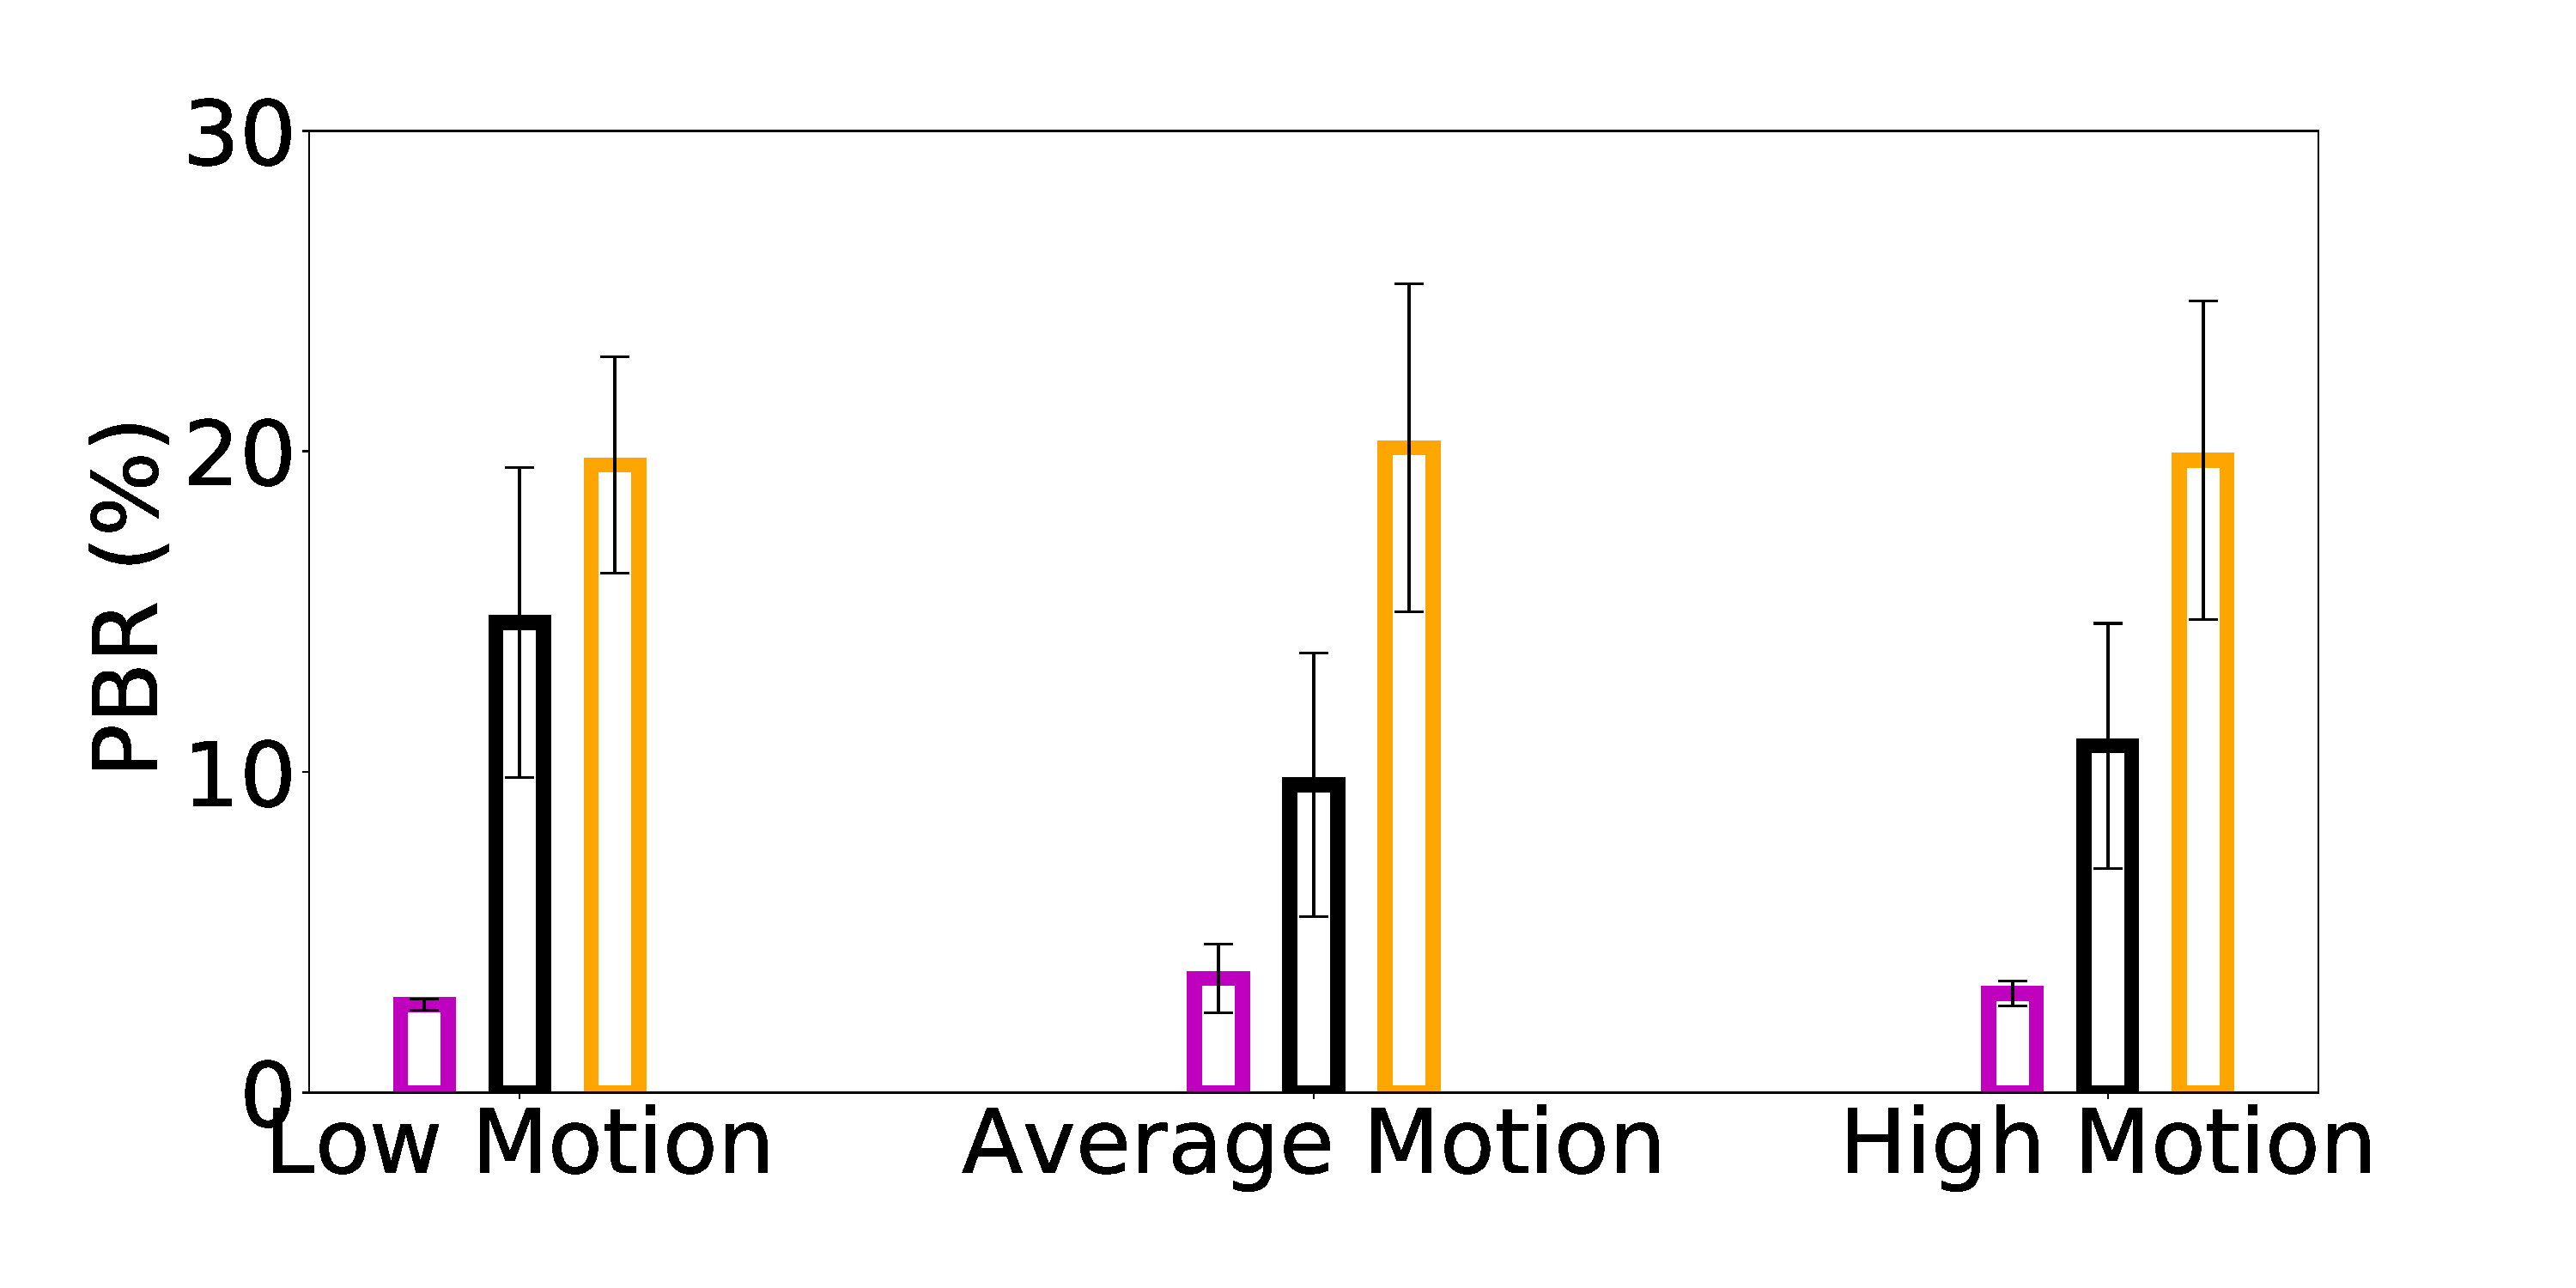
\includegraphics[width=1\linewidth]{sections/network-work/content-bitrate}
        \caption{Content and Motion}
    \end{subfigure}
    \begin{subfigure}[b]{0.33\textwidth}
        \centering
        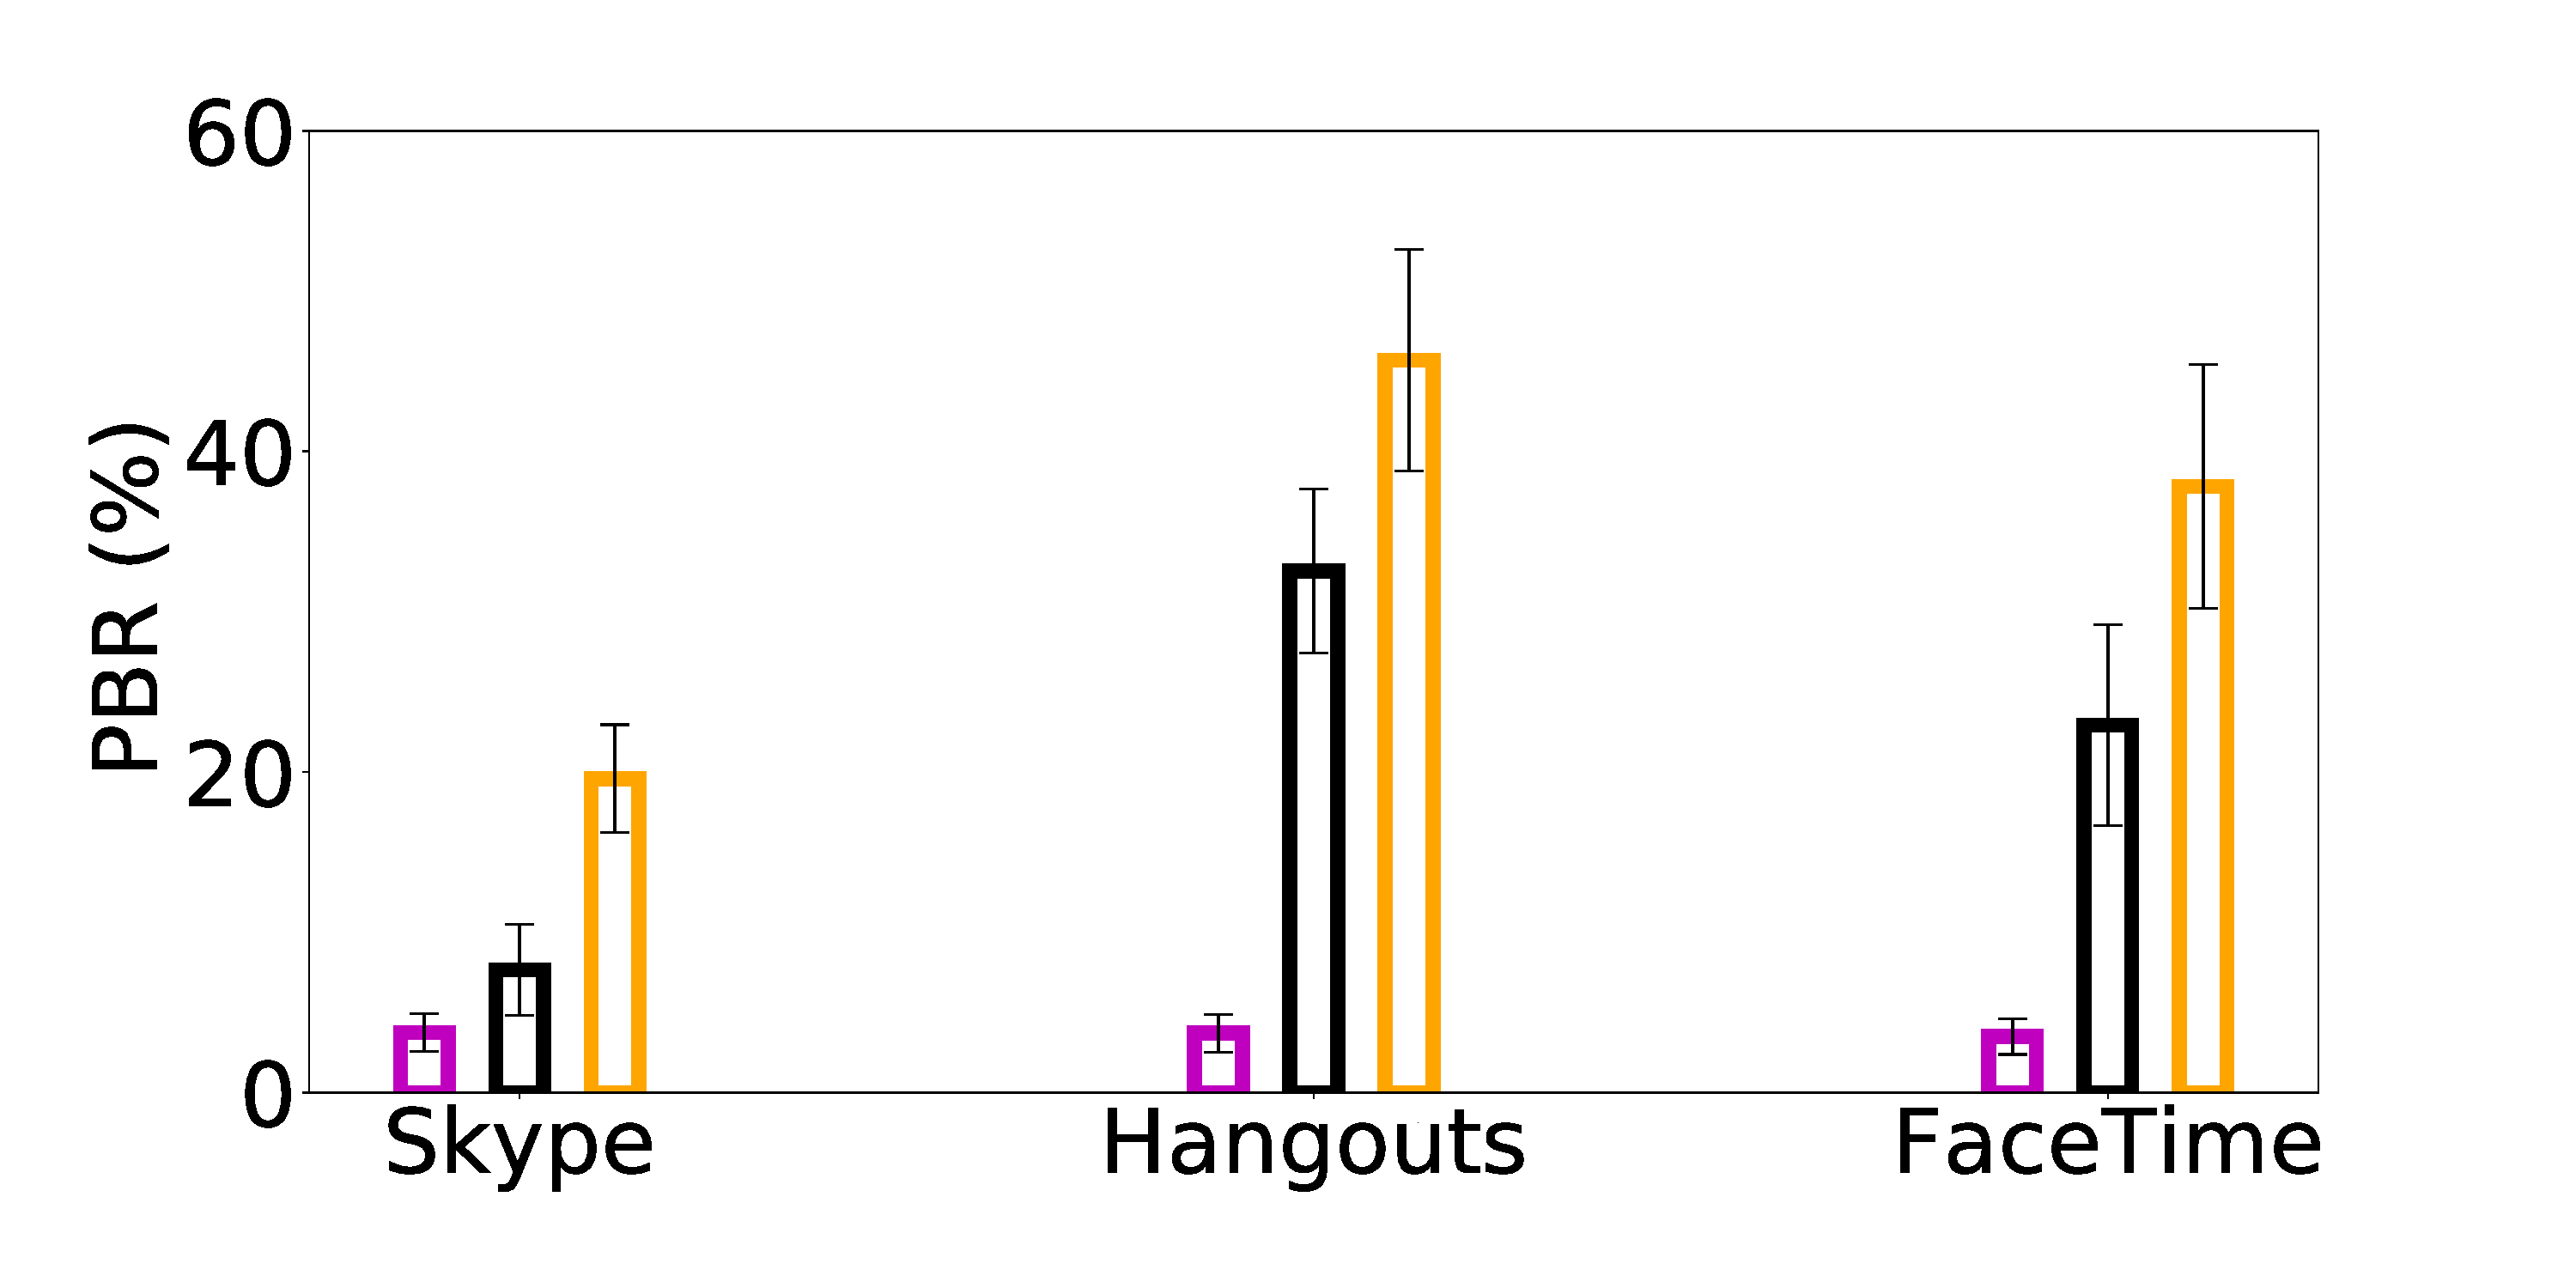
\includegraphics[width=1\linewidth]{sections/network-work/app-bitrate}
        \caption{Applications}
    \end{subfigure}%
    \begin{subfigure}[b]{0.33\textwidth}
        \centering
        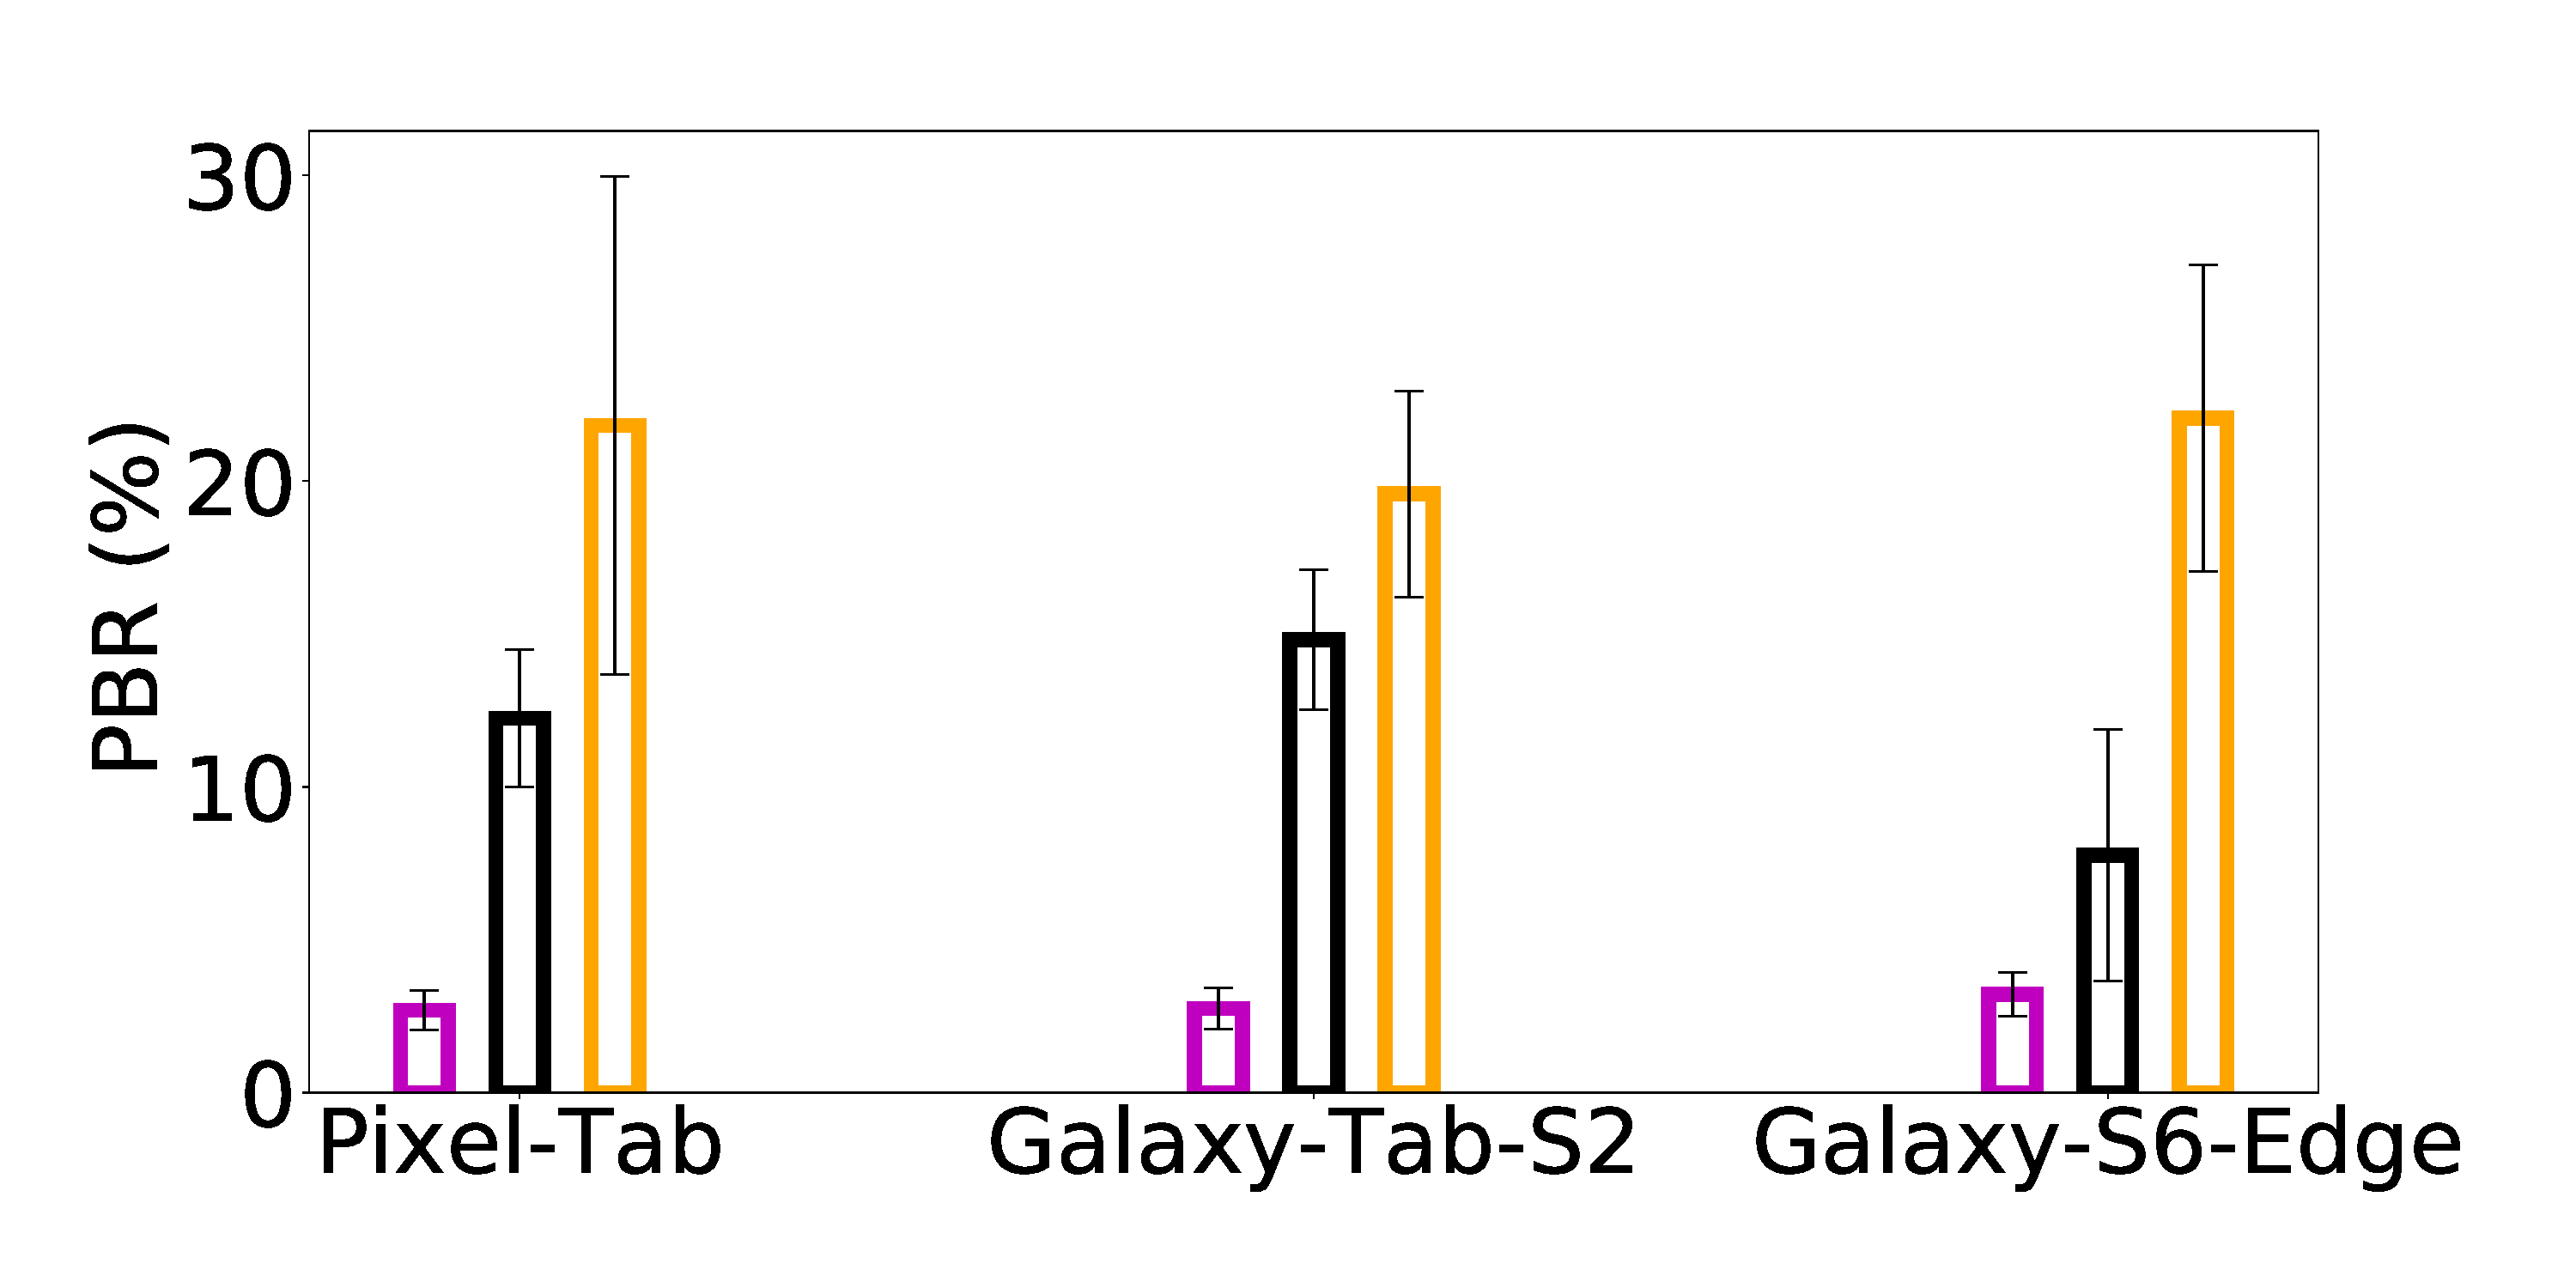
\includegraphics[width=1\linewidth]{sections/network-work/dev-bitrate}
        \caption{Devices}
    \end{subfigure}

     \begin{subfigure}[b]{0.33\textwidth}
        \centering
        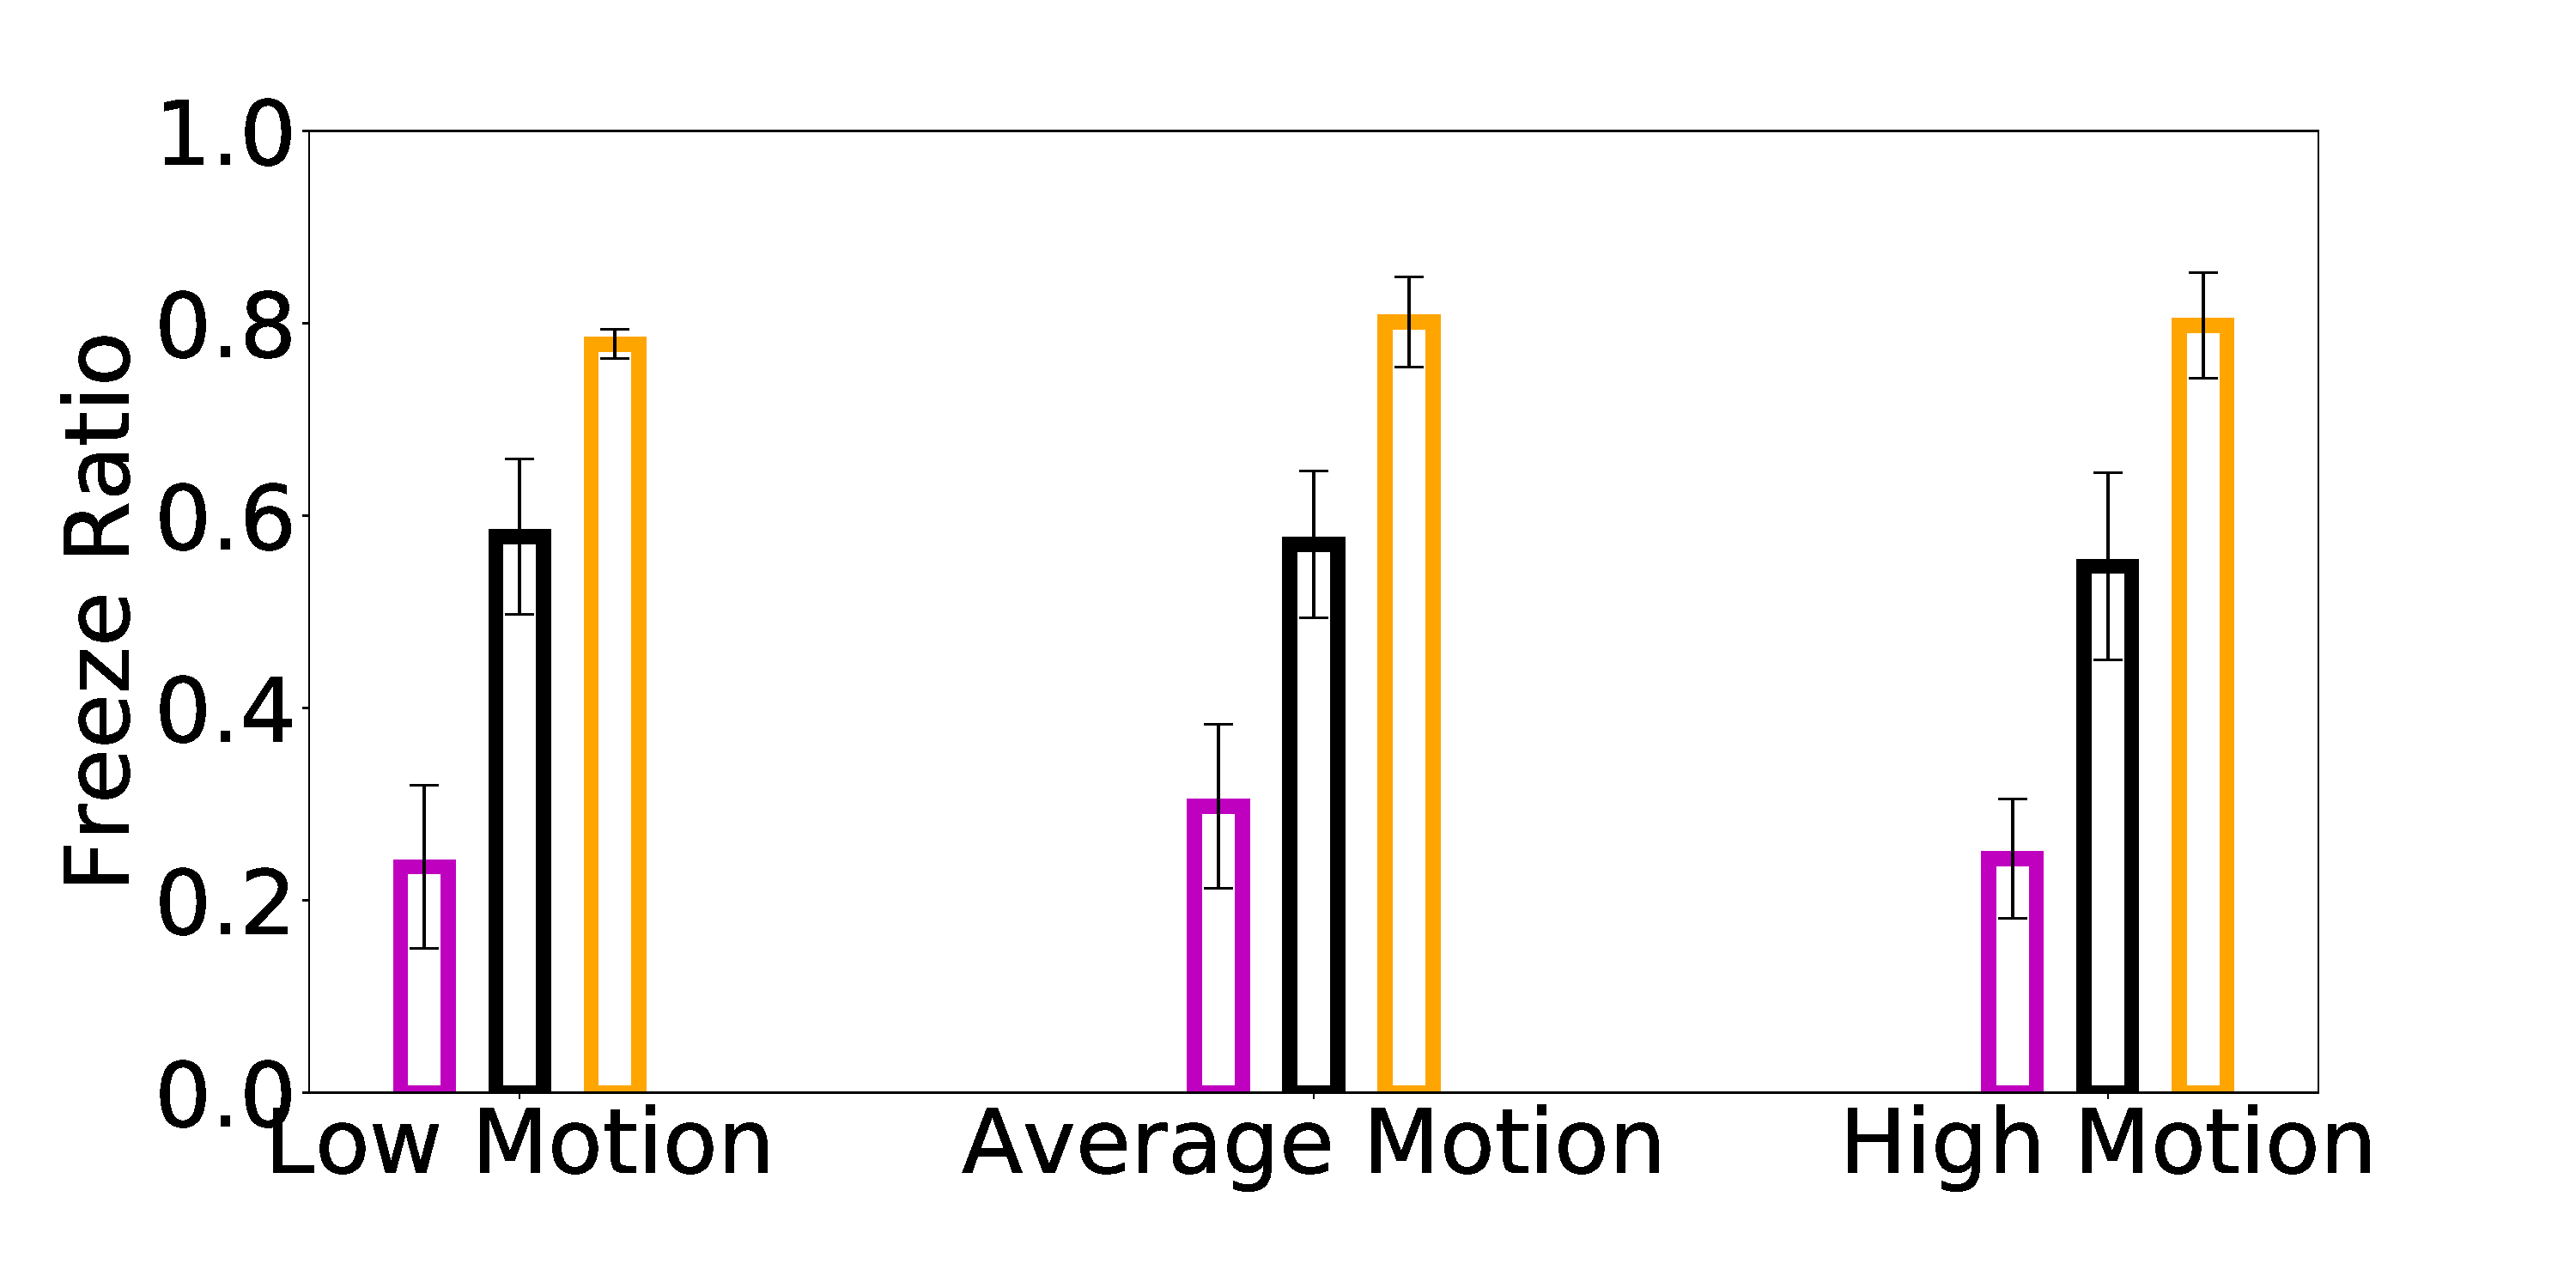
\includegraphics[width=1\linewidth]{sections/network-work/content-stutter}
        \caption{Content and Motion}
    \end{subfigure}
    \begin{subfigure}[b]{0.33\textwidth}
        \centering
        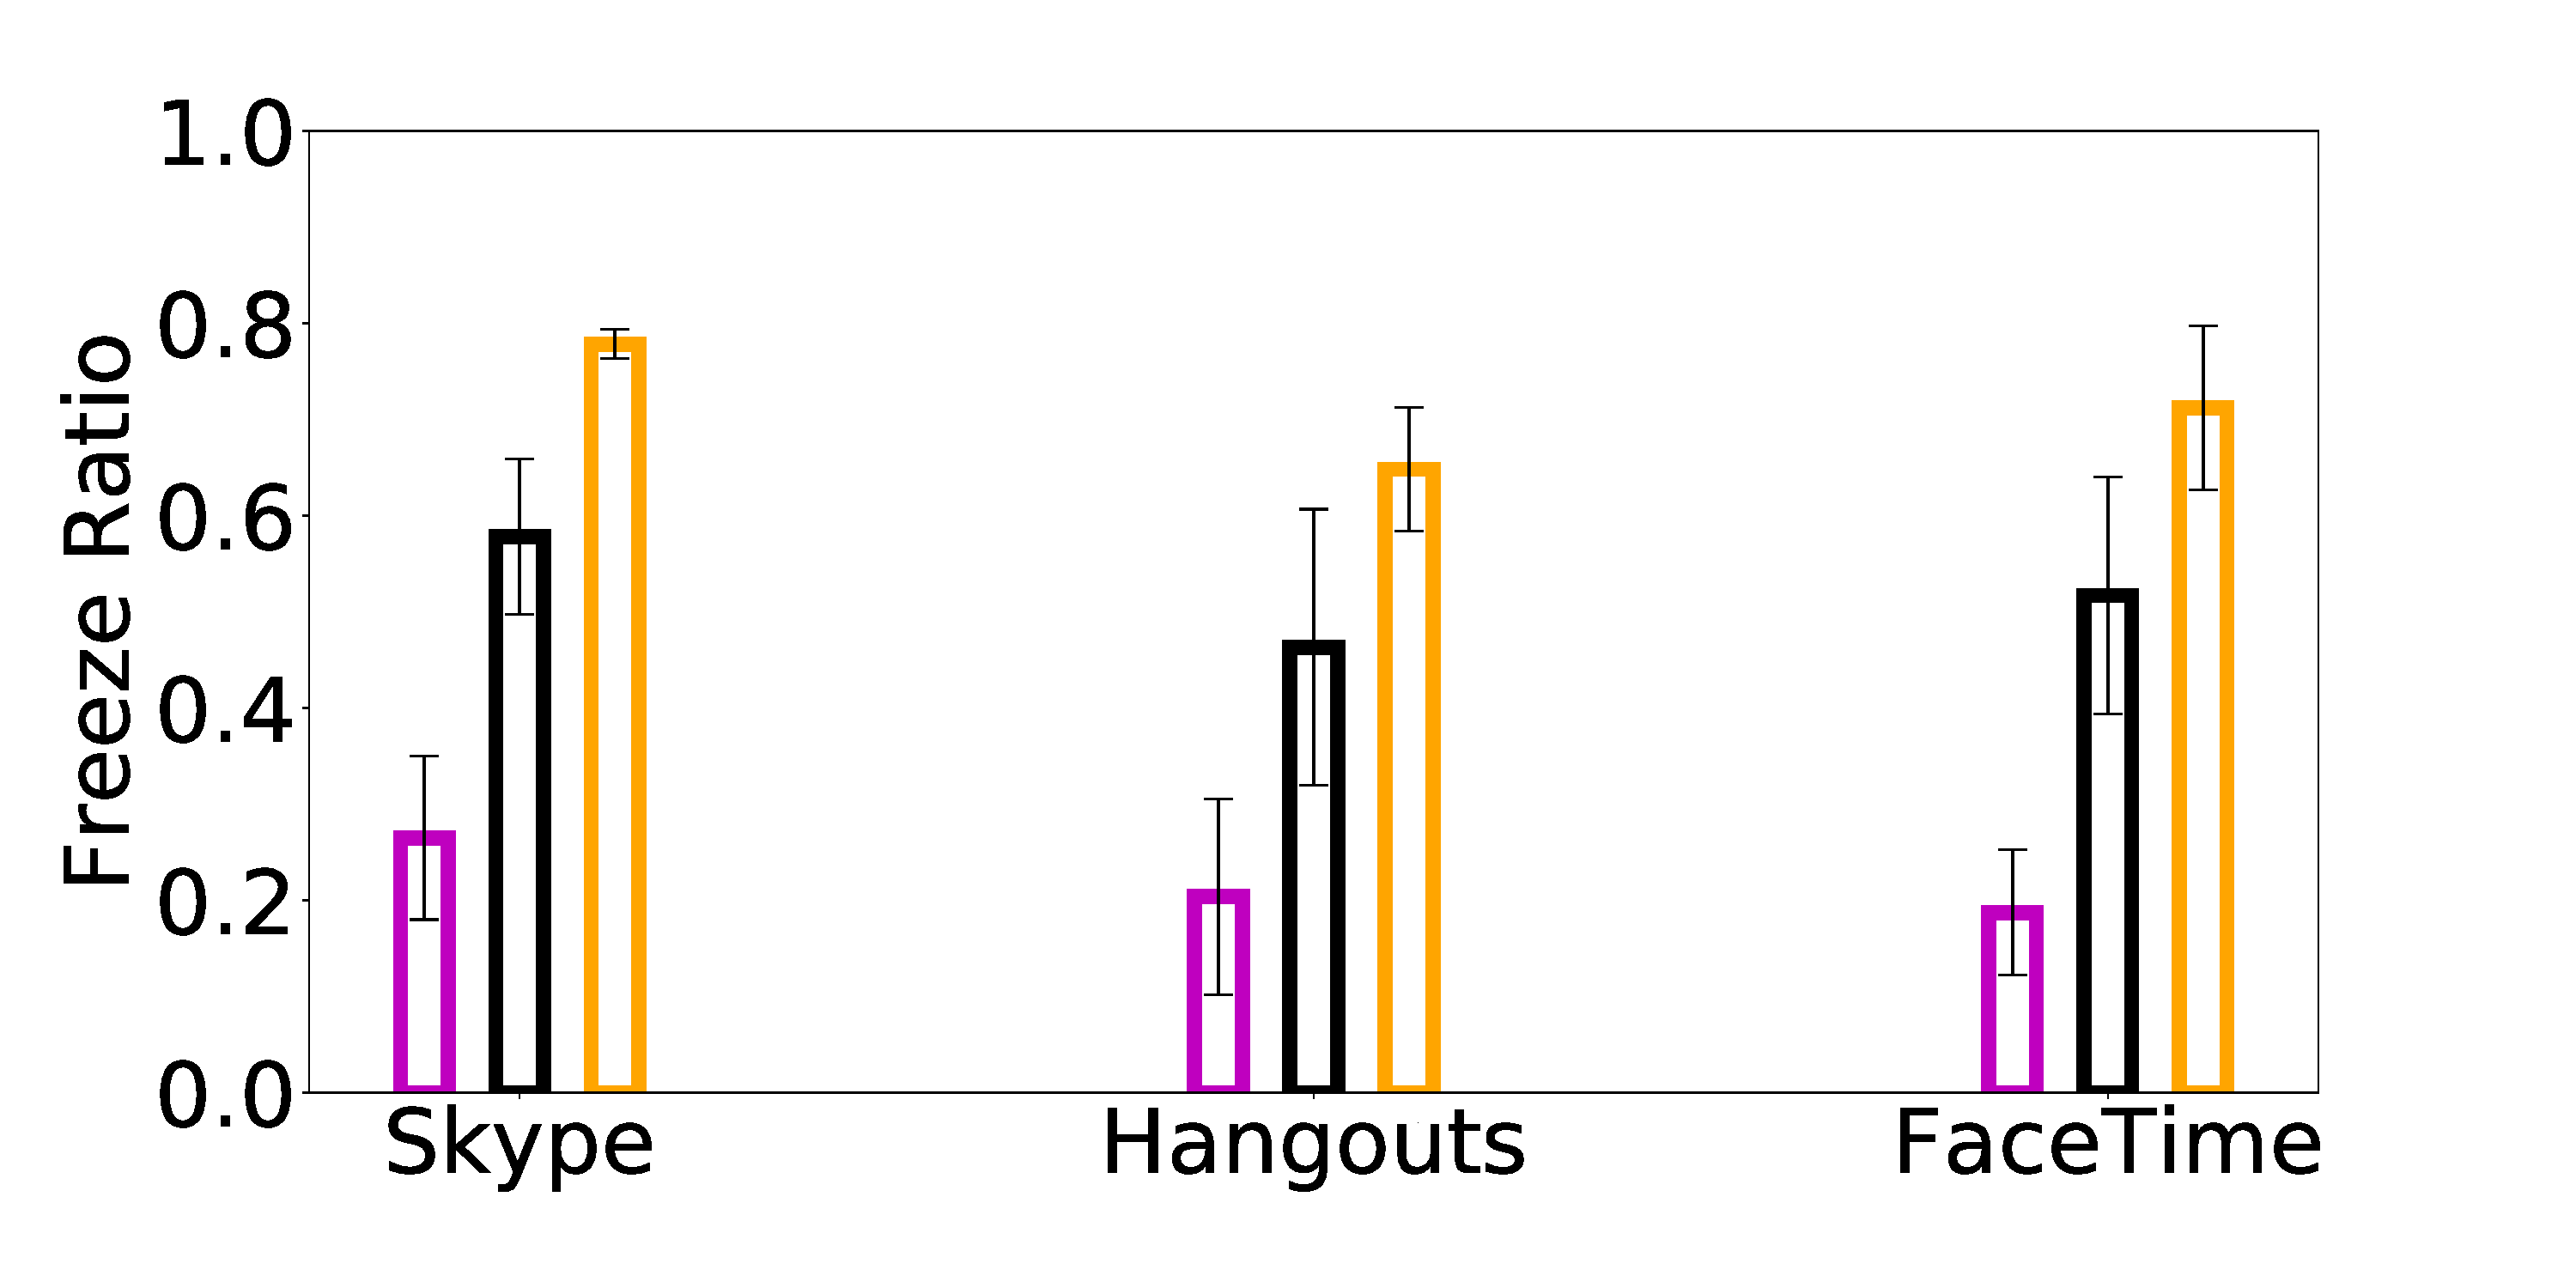
\includegraphics[width=1\linewidth]{sections/network-work/app-stutter}
        \caption{Applications}
    \end{subfigure}%
    \begin{subfigure}[b]{0.33\textwidth}
        \centering
        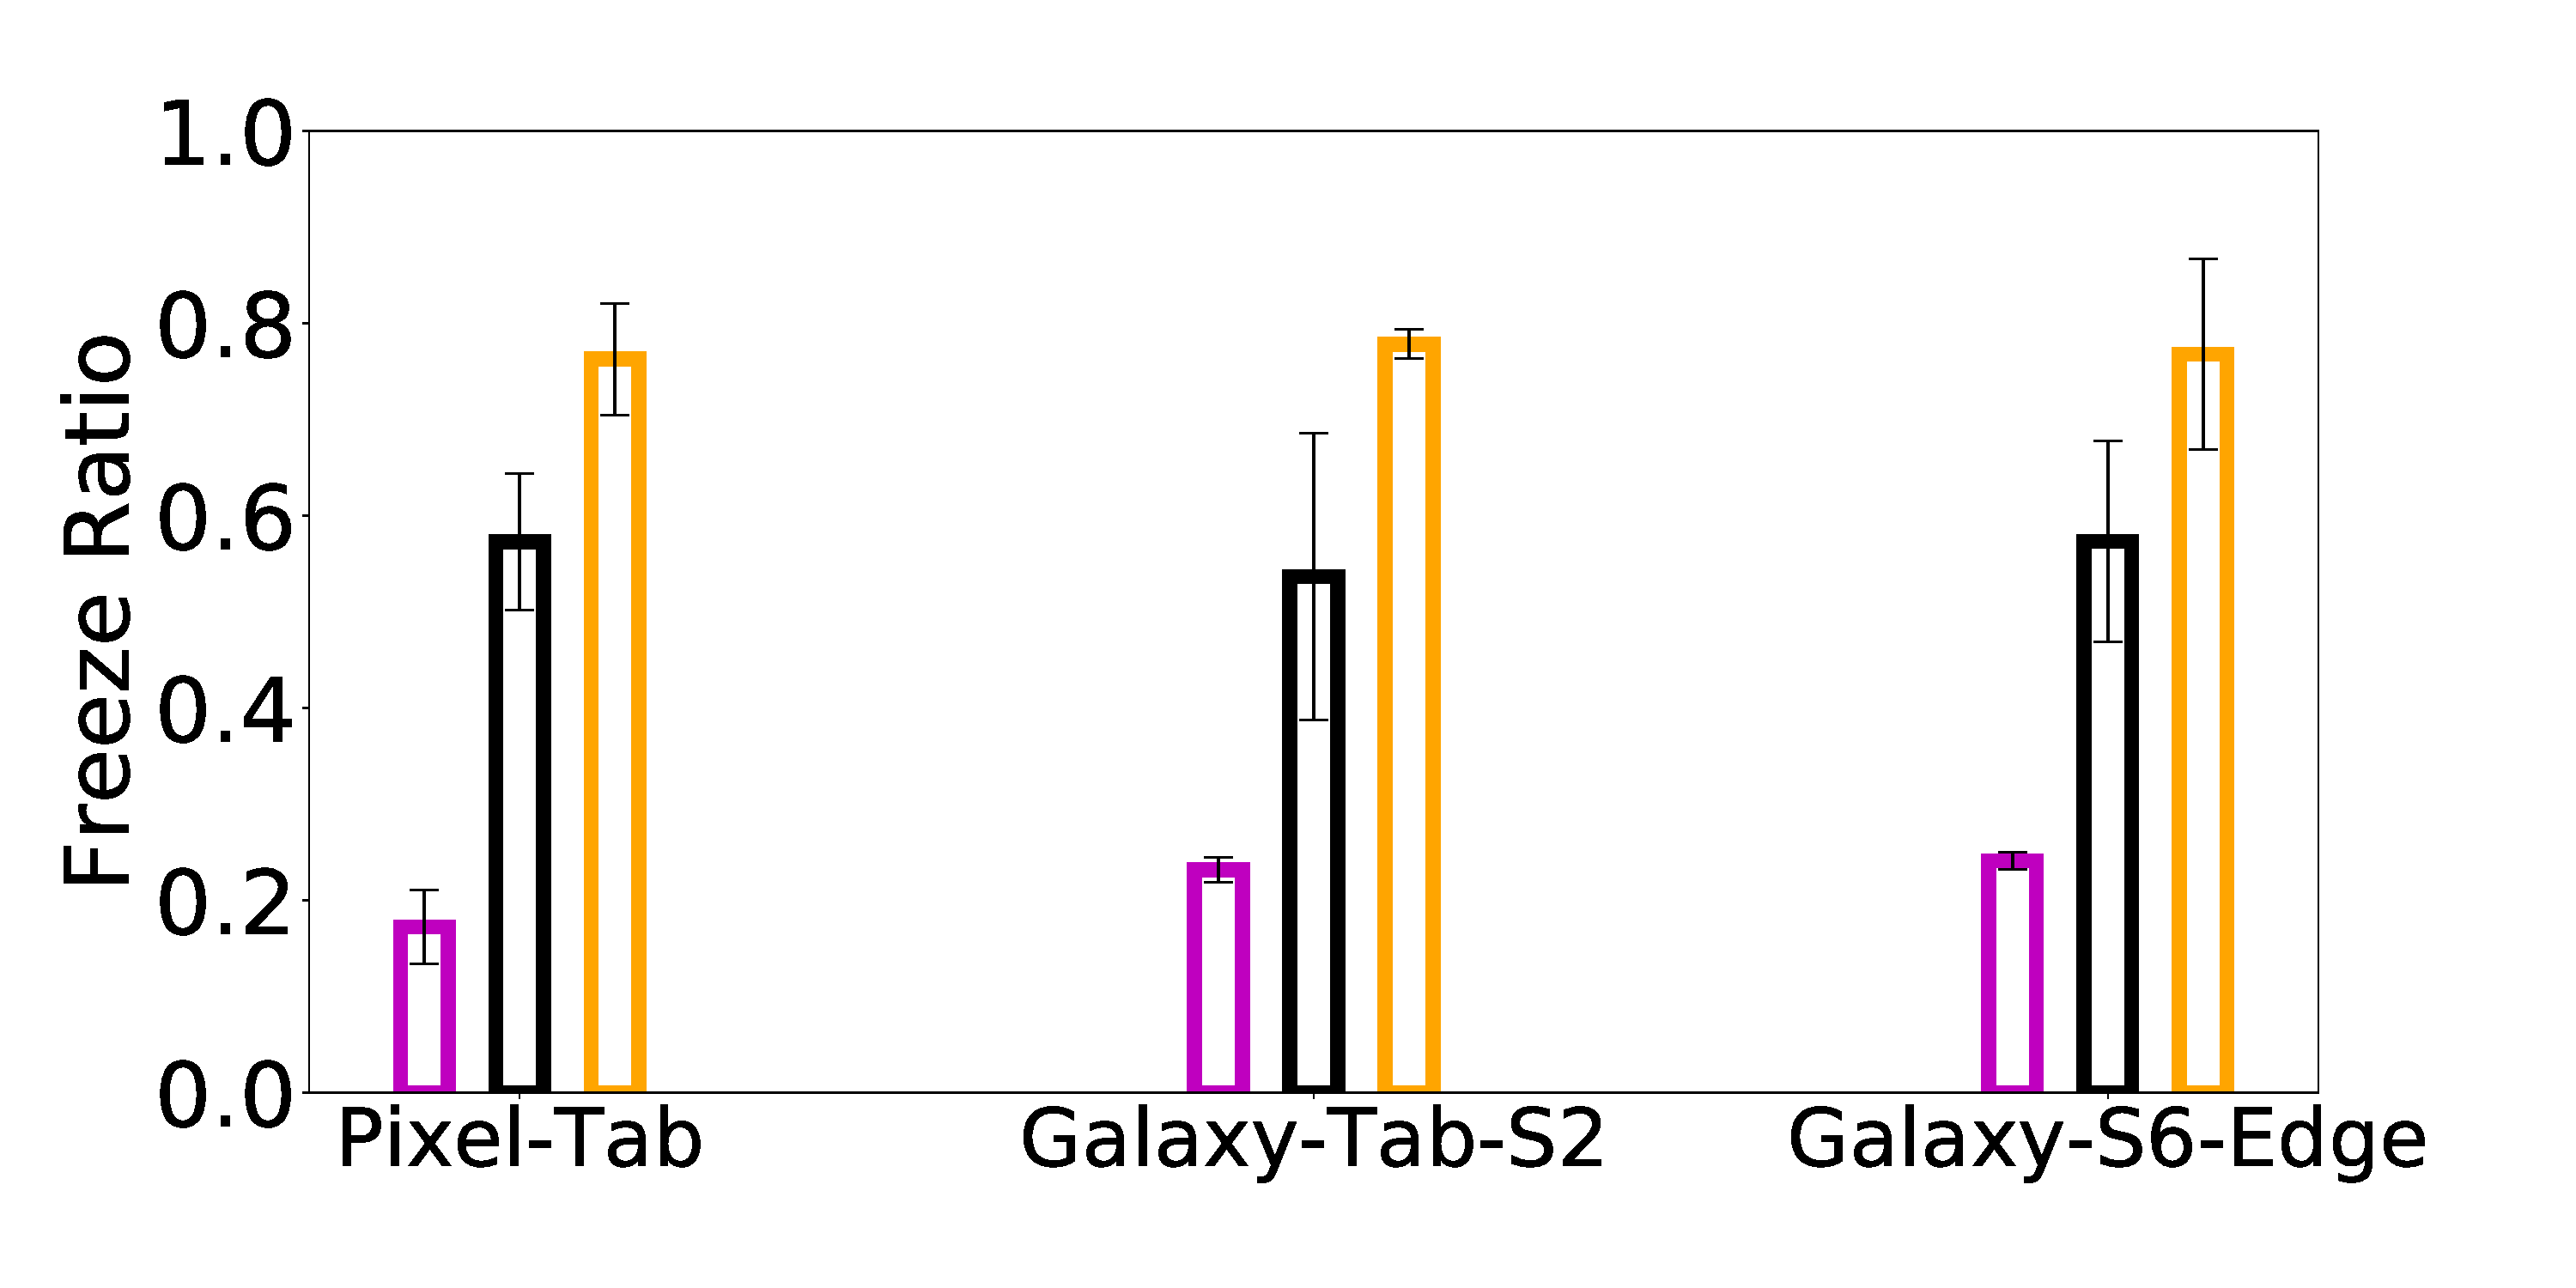
\includegraphics[width=1\linewidth]{sections/network-work/dev-stutter}
        \caption{Devices}
    \end{subfigure}
    \caption{PBR and Freeze Ratio for different videos with respect to content, application and device settings. Results for diverse network conditions are shown (from bad, average, good).}
     \label{fig:measurements}
     \vspace*{-1em}
\end{figure*}

\noindent \textbf{Network conditions:} As we experiment real-time with interactive applications (Skype, Hangouts, FaceTime), we need to emulate real user experience under any condition and to obtain samples with MOS values of all levels (1--5). Hence, we conduct tests with ideal network conditions and with throttled network. To create average and bad network conditions, we use Linux utility \texttt{tc} and we introduce hundreds of ms of delay, packet loss (10--20\% ensuring that the call is setup), or low bandwidth (2--10 Mbps).  

\noindent \textbf{Test video sequences:} We use the same 20 test video sequences as in Section \ref{MOTIVATION}. 
We collect these videos  from Xiph media \cite{xiph2008org} and YouTube. We select 20 representative videos that contain different types of motion and content.
All videos are downloaded in Full HD (1920x1280) resolution.
%Our automated Telephony client is restricted to few container formats, so we could not host raw videos but had to encode into AVI container format. 
%While converting $y4m$ into $AVI$, we use $ffmpeg$ to extract $fps$ and $bitrate$ of compression. We exploit these video coding artifacts in classifying the motion present in the video. We observe motion is directly proportional to $fps$ and inversely proportional to output $bitrate$ of video coding. Table~\ref{tab:table2} gives statistics corresponding to motion in the video. All the videos are of High Definition (HD ) resolution with $16:9$ aspect ratio and $4:4:4$ color space format. The videos are encoded under same encoding parameters such as libx264 video codec, quantization parameter (25), YUV $4:2:0$ output color space format.

\subsubsection{Our QoE Metrics}
%In this section, we describe our QoE metrics.

\noindent \noindent \textbf{PBR:} 
Video bitrate has been considered a standard metric for perceptual quality of video \cite{zhang2012profiling, chakraborty2016exbox}.
We compute the bitrate of recorded videos as a QoE metric. Typically, the bitrate is lower for low resolution video and higher for high resolution video and depends on the level of video compression.
Therefore, we capture video blur with \texttt{encoded bitrate} by compressing the recorded video. 
We employ the observation that the blurrier the video is, the higher compression efficiency is. 
However, we find that the bitrate metric is sensitive to motion in the video, because the block movement for high motion videos is very high and it is low for low motion videos. This results in different encoding bitrates. 
As described in Section \ref{label:background}, low motion videos take advantage of inter-frame prediction, which makes the encoded bitrate motion-sensitive. 
Therefore, we use intra-coded bitrate by \emph{disabling the inter frame prediction while compressing video.}
We experiment with different encoding parameters like quantization parameter (QP) and de-blocking filter techniques and we choose high QP value (30) while coding, to get large bitrate difference when encoding high- and low-quality videos. 
To achieve robustness to video content, we compute the \emph{relative change between the recorded bitrate and  the intra-coded bitrate of the compressed video.} We define this change as the perceptual bitrate (PBR), as it only captures quality of the image. Since we calculate PBR on the recorded video, we do not need a reference video, hence PBR is a no-reference metric.

We validate the PBR metric with respect to the same 20 videos used to compute blur using DCT coefficients in Section \ref{MOTIVATION}.
We create two sets of videos with high and low quality and record them during a Skype call under best network conditions.
This experiment aims to validate our blur capturing metric, hence we avoid video freezes by sending low quality videos over best network conditions.
Fig. \ref{fig:ourblurdetection} shows PBR for both low and high quality videos.
We observe a PBR larger than 20\% for low quality videos, whereas PBR is smaller than 5\%  for high quality videos.
Unlike blur detection using previous methods, we see a clean separation of average PBR between low and high quality videos. Therefore, PBR can be used to detect blurriness in videos without any ambiguity.

%In addition to PBR, we also compute gradient of PBR (PBR-G). This denotes the number of times the quality level is changed in a given video call. This variation happens because of adaptive video-streaming solutions. More specifically, the clients estimate the bandwidth and request corresponding video quality from server. If the network conditions change frequently, quality of video also fluctuates frequently. Because of this high variability in quality, the users get dissatisfied easily. Therefore, we use \texttt{PBR} and \texttt{PBR-G} metrics to capture spatial artefacts of QoE.

\noindent \textbf{Freeze Ratio:} As described in Section \ref{label:background}, freeze ratio is another important QoE artefact. 
Freeze ratio is the number of repeated frames over total frames in a given window, i.e., it denotes the amount of time the video is paused because of network disturbance. 
We use Ffmpeg's \textit{mpdecimate} \cite{ffmpeg} filter in calculating freeze ratio. 
The \textit{mpdecimate} algorithm works as follows: The filter divides the current and previous frame into 8x8 pixels blocks  and computes sum of absolute differences (SAD) for each block. 
A set of thresholds (\textit{hi, lo and frac}) are used to determine if the frames are duplicate. 
The thresholds \textit{hi} and \textit{lo} represent number of 8x8 pixel differences, so a threshold of 64 means 1 unit of difference for every pixel. A
frame is considered to be duplicate frame if none of the 8x8 blocks yields SAD greater than a threshold of \textit{hi}, and if no more than \textit{frac} blocks have changed by more than \textit{lo} threshold value. 
We experiment with several other error methods such as MSE and MAD, but we notice similar results among all three, thus we choose SAD for minimal computation overhead. 
We use threshold values of 64*12 for \textit{hi}, 64*5 for \textit{lo} and 0.1 for \textit{frac} for all our experiments. 
The metric does not work if the entire video is having a still image (for instance a black screen throughout the video). 
However, we think that it is a reasonable assumption that most of video telephony applications do not generate such video content.

In addition to freeze ratio, we also compute length and number freezes in video. We define a freeze if the video is stalled for more than one second. We observe that users do not perceive the stall when the length of freeze is very short or if there are very few such short freezes in the video. Therefore, we employ \texttt{freeze ratio, length and number of freezes} metrics to capture the temporal artefacts of QoE.

\subsubsection{Micro-Benchmarking of Video Artefacts}
In this section, we show the scalability of our metrics through measurements across different applications and devices. As described above, we use a total of 4 metrics: PBR, freeze ratio, length and number of freezes in the video. For brevity, we show measurements for only PBR and freeze ratio. We find similar trends with other metrics as well. We measure these metrics with 6 different videos from the 20 videos described in Section \ref{MOTIVATION}, that cover high video-motion and content diversity. These experiments are run on Skype and Samsung Galaxy Tab S2 unless otherwise specified. All videos are recorded under Full HD (1920x1280) resolution with 60 Fps. Each experiment consists of 20 minutes video call with a total of 18 hours of video recordings. The videos are recorded under different network conditions to obtain different video quality  levels. We use the following network conditions: good case (0\% loss, 0 latency and 100 Mbps bandwidth), average case (5\% loss, 100 ms and 1 Mbps bandwidth) and bad case (20\% loss, 200 ms, and 512 Kbps bandwidth). Fig. \ref{fig:measurements} shows PBR and freeze ratio across different applications and devices. Our observations are the following.



\noindent \textbf{Video Motion and Content Diversity:} 
The average PBR for best network conditions is always smaller than 5\%. PBR is larger than 20\% under bad settings (see In Fig.~\ref{fig:cont-pbr}). 
The average freeze ratio for best network conditions is smaller than 0.3 and for bad conditions, it is larger than 0.8 (Fig.~\ref{fig:cont-st}). 
We observe that both PBR and freeze ratio are highly impacted by network conditions and follow same trend with network quality irrespective of content and motion in the video.
Therefore, the videos can be labeled accurately because of clear separation between network dynamics.

\noindent \textbf{Application Diversity:} 
In Fig.~\ref{fig:app-pbr},~\ref{fig:app-st}, we present PBR and freeze ratio for three applications: Skype, FaceTime and Hangouts.
For Skype, we observe an average PBR of less than 5\% with good network and 20\% with bad network. 
Whereas, both FaceTime and Hangouts reach more than 40\% PBR under bad network. 
This discrepancy is due to application logic: Skype does not compromise quality of video, hence low PBR. But, this causes Skype video calls to be stalled more frequently compared to other applications under bad network scenarios. Whereas,  bitrate adaptation of FaceTime and Hangouts sacrifices quality to provide temporally smooth video. 
Moreover, quality and bitrate are highly impacted by the underlying video codec the application uses. In our experiments, Skype uses H.264 whereas Hangouts uses VP8. We observe that using different video codecs and adaptive bitrate (ABR) algorithms impacts video quality during call.

The freeze ratio for Skype is similar to FaceTime and Hangouts. However, as network conditions worsen, Skype yields more freezes compared to other applications. Despite the additional freezes, the average freeze-ratio for Skype is only 0.1 larger than other applications. This is due to the longer freezes of FaceTime and Hangouts than of Skype.

\noindent \textbf{Device Diversity:} We aim to devise a model that is independent of the device that runs video telephony. Our metrics should capture similar video QoE on different devices given that screen recorder and network conditions are the same. To this end, we evaluate our metrics on three devices: Samsung Galaxy Tab S2, Samsung Galaxy Edge S6 and Google Pixel Tab. 
In Fig.~\ref{fig:dev-st},~\ref{fig:dev-pbr}, we observe that both PBR and freeze ratio show same distribution under different network settings on all devices. Hence, our metrics are device independent.
